\chapter{Implementation}
\label{cha:impl}
This chapter introduces the implementation of the approach in detail. The details contains the feature selection, the similarity calculation, the logistic regression, the clustering algorithm, the practical issues and the Java implementation. The practical issues are the optimizations for the approach.
 
\section{the Feature Selection}
The target of the inventor identification is to identify if two inventor-patent instances are from the same person or not. In order to do that, some information is used as the features to represent the inventor-patent instances. Extend Flemming's \cite{RePEc:eee:respol:v:43:y:2014:i:6:p:941-955} inventor-patent instance data structure by adding four text features which are extracted from USPTO patent documents. The inventor-patent instance for my master thesis contains 10 features. These features describe the inventor information and the patent information for the inventor-patent instance. These features have different data types, such as the string and the number. In this section, the features and their data structures are introduced in detail.

%For my master thesis, the raw patent information comes from the USPTO. Thanks to the Flemming's research\cite{RePEc:eee:respol:v:43:y:2014:i:6:p:941-955} before and  free access to  patent database built by him and his colleagues, I could easily extract a lot of useful information of the patents from 1975 to 2010 such as the inventor names, assignee information, location information, technology class and the co-inventor information. Except that,  I use the Patent Full-text Database(Patft) API to extract the texts of the patent such as the abstract, claims and description. These information are classified into two categories, patent information and inventor information. Patent information includes the assignee information, technology class, co-inventors and the texts. The inventor information includes the last name, first name and the location of the inventor. These information is used as the features to represent the inventor-patent instance. 

\subsection{Names of the Inventors}
The name of the inventor always contains a last name and a first name. Because not every inventor has a middle name, the middle name is omitted for my approach. The original expressions for the inventor names are strings. In order to improve the accuracy, the names of the inventors are preprocessed. The punctuation in the names is removed and all the letters of the names are transformed into capital letters. For each inventor-patent instance, two transformed strings are used to represent the first name and the last name of the inventor. 

%Names of the inventors should be the most important feature of the patent-inventor unit, although the non-uniqueness of the form of names and the duplicate names cause a lot of troubles and it is possible that some inventors may change his names during his life, but this case seldom happens. So it's assumed that each inventor usually has only one name for himself. Although, it's possible two inventors have the same name especially for some very common name such as the "John Smith", in the contrary two inventors are two different persons if they have totally different names. For example, if one inventor is called "John Smith" and another one is called "Peter Green", it's almost one hundred percent true that they are two different persons. This good natural property of the names makes it as the most important feature for inventor identification. From the patent database or the patent document, the inventor names could easily extracted. For my approach, I only use the last name, the first name and omit the middle name because not every one has a middle name. The data structure of the names are two strings. For many approaches, some rules have been applied to format the strings of the name. This behaviour sometimes do some harms for identification and is complex. Although the non-uniqueness of the form causes troubles, it is obvious the different forms of the same names should also be similar. For example, "John Smith" and "J. Smith" are similar strings. Based on that, for my approach, the original expression of the names would be used and a string similarity calculation would be used to measure the similarity of the names of the inventor.


\subsection{the Assignee of the Patent}
Assignees are the organizations such as some people, some companies and some institutions which own the patents. The patents from the same inventor are usually assigned to the same assignees. It is true that the assignees of the patents from the same inventor may be different. For example, some academic researcher may give the ownership rights of his patents to his research institution or some companies. On the other hand, some big organizations usually own many patents of different inventors. However, considering that the inventors usually cooperate with a limit number of the assignees, the assignee information is a good indicator to distinguish the patent inventors. The assignee information contains a string for the assignee name and an assignee code. The assignee code in the Flemming's database is extracted from the National Bureau of Economic Research (NBER). The assignee name like the names of the inventors doesn't have a unique form. So the assignee code is the first choice to check if two assignees are same or not. As not every assignee has an assignee code, the assignee names are still used to distinguish the assignees if the assignee codes are not available.  


\subsection{the Location of the Inventor}
The raw patent document contains the city, the state, and the country information for each inventor. Because the inventors usually stay in a specific area, the close locations for inventors can be another indicator to show the probability that they are the identical person. It's not smart to compare the city, the state and the country, because it's very difficult to measure the closeness by simple comparison. For example, the cities from two different states sometimes have a smaller distance than the cities from the same state. The location information which is used to represent the inventor-patent instance contains the longitude, the latitude and the country as the Flemming's representation \cite{RePEc:eee:respol:v:43:y:2014:i:6:p:941-955}. The longitude and the latitude could be extracted from some data sources such as the US Board on Geographic Names used by Flemming \cite{RePEc:eee:respol:v:43:y:2014:i:6:p:941-955}. The country information is kept because if the inventors are from different countries, it shows a high probability that their nationalities are different. If the inventors are in the same country, the longitude and latitude are used to compute a distance between the inventors.


%As the inventor may change the locations, a simple comparison of the cities, the states and the countries would be not precious. As an assumption, the inventors locations usually are closed to each other. A dichotomous result of these information couldn't measure the closeness of these locations. The distance would be a good choice for the measurement. In order to compute the distance, the longitude and the latitude should be used. The closer are the locations, the inventors have a higher probability to be the same person. My approach uses the Flemming's method of the location comparison as a reference. The location information is not a strong evidence to identify the inventors. Because in the same city especially for some large cities, there are a lot of inventors. What's more, the colleagues usually have the close locations. For my approach, the longitude, latitude information and the country information from the Flemming's database would be used as the locations of inventors. The longitude and latitude information would be used to calculate the distance if the inventors are in the same country.

\subsection{Technology Classes}
The technology classes represent the fields of the patents. The inventor usually focuses on some fields such as computer science, chemistry or economic. Although the inventors may cover several fields, the patents from the same inventors are usually from the same fields. In addition, the inventors with the same name focusing on the same fields are not common. Therefore, the technology class can be used as an index to distinguish the inventors. According to the technology class definition of the USPTO, the technology classes of the patents are classified into main-classes and sub-classes. A main class contains a list of sub-classes. Although classes usually have some relationships such as the computer science and math, the relationship is difficult to measure. The semantic of the class is ignored for the approach. The classes are represented by numeric codes. The code meaning can be found in the USPTO technology class website \footnote{US technology class number with title: \url{http://www.uspto.gov/web/patents/classification/selectnumwithtitle.htm}}.
Each inventor-patent instance contains a list of main class codes. Each main class may contain a list of subclasses if the subclasses are available.

%So the technology class could also be used as an index for the inventor identification. Different person would focuses on different fields. And it's assumed that even for the inventors whose names are same also seldom focus on the same fields. But as we know, there are a lot of inventors in the same field. However, we should also know that the inventor may also cover several fields. These phenomena weaken the importance of the technology class. According the technology class definition of USPTO. The technology classes are divided into main class and subclass. Each class contain a lot of sub classes. For example, the main class of the data processing contains the histogram distribution, probability determination and etc. So for each patent-inventor pair, a main class list and a subclass list would be used to describe the technology class. For my approach, the relationship between different classes is omitted. For example, the data processing and the database could be considered similar. But as the classes contains a lot of fields and it's difficult to identify these relationships. However, the sub class would have a larger importance than the main class  when we compute the similarity of the technology class between two patent.

\subsection{Co-inventors}
A patent usually contains several inventors. The inventor-patent instances generated from the same patent contains one inventor from the inventor list of the patent. The other inventors are considered as the co-inventors. The inventors usually cooperate with their colleagues. The inventors who share a large number of co-inventors have a high probability to be the same person. Co-inventors are stored as a list of strings which represents the inventor names. Because the raw inventor-patent instance doesn't contain the co-inventor feature, a query by using the patent number as a keyword for each inventor-patent instance is applied. The inventors of the returned inventor-patent instances whose names are different from the inventor name of the specific inventor-patent instance are used as the co-inventors. Co-inventors are used as a good indication to help us distinguish the inventors who have the same name, but it cannot help us to distinguish the colleagues as they usually share the same co-inventors.


%Usually, the patent has several inventors. For the patent-inventor pair, only one inventor is considered and the other inventors are considered as the co-inventors. The co-inventors index based on the assumption, inventor usually cooperate with some specified persons. So if it is found that two inventor always cooperate with the same persons, it has a high probability to be the same person. Although this index shows a promising strong evidence to identify the inventors, the colleague phenomenon would weaken this index role during the identification of inventors. The co-inventor list often contain more than two inventors. If we choose the inventor and one of his co-inventor and check their patents, we would found they usually have many same co-inventors. The co-inventor information for my approach is stored as a list of the patent inventor name strings. When we compare the co-inventors, we just check the size of the intersection of the two patent inventors. 

\subsection{Texts of the Patents}
The text of the patent is extracted by using the Patent Full-Text Serach Engine (Patft).  According to the format of the patent documents, the content of the patent can be divided into four basic parts: the title, the abstract, the claim and the description. The title usually contains several words to briefly describe what the patent it is. The abstract is a short paragraph to give an overview of the patent. The claim describes the extent of the patent. The claim is of the utmost importance both during prosecution and litigation alike. The description usually gives the details of the patents. For the legal reasons, the texts of the patents of the recent years usually are not allowed to be extracted. My experiment of the text extraction shows that most of the texts of the patents from the Flemming's database are available. Dealing with the text data is usually related to the text mining techniques which can be considered as the natural language processing. For my approach, the texts are transformed into vectors which are easily used to compute the similarities. The text similarities  reflect the semantic similarities between patent texts. As it's mentioned, the inventors are usually focusing on some fields. The patents from the same inventor should have big similarities between the texts. The transformation of the texts can be divided into three steps. They are "remove the stop words", "stemming" and "normalized term frequency calculation". 

\begin{itemize}
\item  \textbf{Remove the Stop Words:} In the context of the patent, a lot of common words appear many times such as "a", "an" and "the". For the vector model of the text, the frequencies of a word is used to represent the text. These words are not discriminative. In addition, because these words appear in most of the texts, keeping them does harm to the similarity calculation between two texts. Therefore, these words should be removed from the texts first. Besides that, there are some other words such as the number and Greek alphabet. These words should also be removed from the text.
 
\item  \textbf{Stemming:} Stemming is a technique to reduce the number of the terms of the context by transforming the words into their stems. Because many words have the same meaning and share the same stems, they should be considered as the same term. For example, "Apply" and "Application" or "Describe" and "Description". For my approach, the terms of the texts refer to the stems, not the words. 
 
\item  \textbf{Normalized Term Frequency Calculation:} After removing the stop words and stemming, the term frequencies of the stems are counted for different texts. The frequency is how many times a stem occurs in the text. Considering that different texts from different patents usually have different length. A normalization should be applied after the calculation of the term frequency. The normalization is dividing all the term frequencies by the total number of the stems . For many vector-space models of text, the inverse document frequencies are used as the weights of the stems. However, the inverse document frequencies (IDF) relate to the chosen text sets. The term frequency of the same text may varies a lot if different text sets are chosen. It will also affect the text similarities between the texts. Therefore, IDF is not used for my approach.
\end{itemize}

In addition, the stop words and stems are related to the language used for the patent. For my approach, the stop words and the stems are from the English language because the patents are all from the USPTO. The following text is a small paragraph copied from wiki which describes the RWTH University. The table 4.1 shows the stems, the term frequency and the normalized term frequency by applying the three methods on this paragraph.
\begin{quotation}
\emph{RWTH Aachen University is a research university of technology located in Aachen, Germany. With more than 42,000 students enrolled in 144 study programs, it is the largest technical university in Germany.}
\end{quotation}

\begin{table}

\begin{center}
\begin{tabular}{ | c | c | c |}
\hline
  Stem  & Term Frequency & Normalized Term Frequency \\ \hline
  Aachen & 2 & 0.125 \\ \hline
  Enrol & 1 & 0.0625\\ \hline
  Germani & 2 &  0.125\\ \hline
  Largest & 1& 0.0625\\ \hline
  locat & 1 &0.0625\\ \hline
  program & 1&0.0625\\ \hline
  research & 1& 0.0625\\ \hline
  rwth & 1 &0.0625\\ \hline
  student & 1 &0.0625\\ \hline
  technic & 1 &0.0625\\ \hline
  technolog & 1 &0.0625\\ \hline
  univers & 3 & 0.1875\\ 
  \hline
\end{tabular}
\end{center}
\caption{the Vector Representation Example of the Text}
\end{table}

For my approach, the patent document is divided into the abstract, the claim, the description and the title to be processed separately. There are two reasons for this separation. The first reason is the different importance of these texts. It's obvious that these four texts describe the patent in different aspects. Processing separately increases the accuracy and is more reasonable. The second reason is the length of the patent document. Taking all the texts as one increases the text preprocessing time and results in a long term frequency vector. The longer is the vector, the more time is used to calculate the similarity. 

\section{the Similarity Calculation}
As it's explained before, there are ten features of the inventor-patent instance and each feature has a special data structure. These structures include strings, numbers and vectors. So based on these special data structures, suitable similarity calculation methods should  be designed for them. Because a weight sum of these similarities is used and the ranges of the similarities are different, the normalization of the similarities is also performed for my approach. All similarities are normalized into the range between 0 and 1. In this section, the details of these similarity calculation methods are described.


\subsection{the String Similarity Calculation}
There are a lot of strings used to represent the features of the inventor-patent instances such as the last name, the first name and the assignee name. The string similarity should be designed first and used for different similarity calculation. A simple comparison of the strings by checking the full matching of the strings is not precise because of the non-unique forms of the inventor names which are extracted from the database. The \emph{Levenshtein} distance as an edit distance of the strings is a good solution for that. The \emph{Levenshtein} distance uses the smallest number of the operations as the distance to transform one string to another one. These operations contains the deletion, the insertion and the substitution.  Because most of the strings used in my approach are to represent the names, the different forms of the names from the same person are similar to each other. This method performs well to find the similarities of the strings. Because different strings usually have different length, a normalization should be performed by a division of the number of steps by the maximum length of the strings. The range of the normalized \emph{Levenshtein} distance is $[0,1]$. In addition, the \emph{Levenshtein} distance as a distance function should also be transformed into a similarity value. Therefore, $1-Normalized Levenshtein Distance$ is used as the similarity of the strings. 


\subsection{the Assignee Similarity Calculation}
The assignee information for the inventor-patent instance contains two pieces of data: the assignee code and the assign name. The assignee names in the patent database also don't have unique forms. The assignee code is more precise to check if two assignees are same or not. Unfortunately, the assignee code is not available for every assignee. The assignee names are also used to compute the similarity if the assignee codes are not available. This is also the reason why the assignee names are kept for the assignee feature data structure. When computing the similarities of two inventor-patent instance assignee features, first check the availabilities of their assignee codes. If both of them are available, a simple comparison of the assignee codes is performed. If the assignee codes are same, the assignee similarity is 1 and otherwise is 0. If at least one of the code is not available, the normalized \emph{Levenshtein} distance is used to calculate the difference of the assignee names and use $1-Nomalized Levenshteim Distance$ as the assignee similarity,


\subsection{the Location Similarity Calculation}
The location information contains the longitude, the latitude and the country information. The geographical distance is used to measure the dissimilarities of the location feature. But the unit of the distance is meter or kilometer. A transformation of the distance should be performed. The Flemming's method \cite{RePEc:eee:respol:v:43:y:2014:i:6:p:941-955} to calculate the level of the location similarity is kept for my approach. The Flemming's location similarity has six levels. The higher level means a bigger location similarity. If the two inventors are not in the same country, the level is 0. If the two inventors are in the same country, a distance based on the longitude and the latitude is calculated. The following formula is used to calculate the level.

\[   
L_{Location}(x) = 
     \begin{cases}
       \text{5} &\quad\text{if x}\le5km\\
       \text{4} &\quad\text{if x}\le10km \\
       \text{3} &\quad\text{if x}\le25km\\
       \text{3} &\quad\text{if x}\le50km\\
       \text{1} &\quad\text{otherwise.} \ 
     \end{cases}
\]
\\

After the level calculation, the normalization method is to divide the level value by 5.

\subsection{the Technology Class Similarity Calculation}
The technology class information of the patents contains a main-class code list and a sub class code list. Each sub-class has been assigned to one of the main-classes. Because some patents only contain the main-class lists, the main-class and the sub-class are both used to calculate the similarity of the technology class. My approach keeps the Flemming's method to calculate this similarity again. The technology class similarity contains 4 levels based on how many class codes the inventor-patent instances share. 4 is defined as the maximum feature value. The normalization is performed by dividing the feature value by 4. The sub-class codes of two inventor-patent instances are same only when they are assigned to the same main-class, because sometimes some sub-classes from different main-classes have the same codes. In addition, some different classes have a close relationship. For example, "Histogram Distribution" and "Probability determination" are two different sub-classes but they are similar to each other. However, the relationship between two different classes is difficult to measure. The relationships of the classes are omitted.


\subsection{the Co-inventors Similarity Calculation}
For each inventor-patent instance, the co-inventor feature contains a list of co-inventor names. The similarity computation of the co-inventors is based on how many co-inventors the two instances share. My approach uses the Flemming's method to calculate the co-inventors similarity. The following is the formula.

\[   
L_{Co-inventors}(x) = 
     \begin{cases}
       \text{6} &\quad\text{if x}\ge6\\
       \text{x} &\quad\text{if x} \in \{0,1,2,3,4,5\} \\
     \end{cases}
\]
\\

The level should also be normalized by a division of 6. The counting of the shared co-inventors based on the full-matched co-inventors names. Although it's possible for the same inventor to have several forms of the name, the normalized Levenshtein distance is not used here, because it would cause troubles for some similar names. For example, "Jack" and "Jake" would have a small Levenshtein distance. The similarity calculation of co-inventors aims at finding the exact number of the shared co-inventors,  so the different forms of names are not taken into consideration here.

\subsection{the Text Similarity Calculation}
As it's explained before, the texts such as the abstract, the claim, the description and  the title are represented as normalized term frequency space vectors. The formal definition of the normalized term frequency space vector is the following.
\\
\begin{equation}
\textbf{V}=(v_1,v_2,...v_n) \quad  \sum_{i=1}^n v_i =1
\end{equation}
\\
Computing the similarity between two texts is considered as the similarity between two normalized space vectors. There are several methods to compute the similarity between two vectors such as the Euclidean distance, the Manhattan distance and the cosine similarity. Among these methods, the cosine similarity is used commonly. The cosine similarity between two vectors ($\textbf{U}$ and $\textbf{V}$) is defined as follows:
\\
\begin{equation}
cosine(\textbf{U},\textbf{V})= \frac{\sum_{i=1}^n u_i \cdot v_i}{\sqrt{\sum_{i=1}^n u_i^2} \cdot \sqrt{\sum_{i=1}^n v_i^2}}
\end{equation} 
\\
The figure 4.1 shows a 2D-dimension vector space which contains two vectors. The vector represents the direction from the original point to the specified point. The cosine value of the angle between the two vectors is used as the measure of the similarity of the vectors. When the angle is zero, the two vectors have the same direction and are considered to have the best similarity of 1. Because the term frequencies are large than 0, the cosine similarity would be larger or equal to zero. The similarity of 0 means the vectors are orthogonal to each other. The cosine similarity has a range between 0 and 1. Because of that, the text similarity is not necessary to be normalized again.
\vspace{6pt}
\begin{figure}
\begin{center}
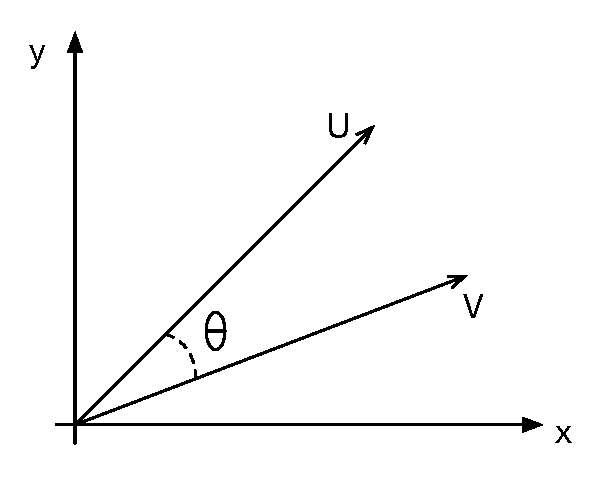
\includegraphics[scale=0.8]{VectorSpace.pdf}
\caption{the Vector Representation Example of the Text}
\end{center}
\end{figure}

\vspace{6pt}

\section{the Logistic Regression}
The logistic regression is a machine learning algorithm to deal with the classification problem. The classical logistic regression is a binary classification and it can be extended to the multi-classification by using the softmax function. The inventor identification problem can be considered as a matching problem. The training data for the logistic regression is generated by using the pairs of the inventor-patent instances with a label indicating the matching state. For each pair of the inventor-patent instances, the similarities based on different features can be calculated according to the methods introduced in the previous section. The logistic regression for my approach is to find suitable values for the weights and threshold. In this section, the basic concept of the logistic regression, the data transformation and the training process of the logistic regression are introduced.

\subsection{the Logistic Regression}
The classical logistic regression is a popular model for the binary classification. Usually, an input vector $\textbf{x}$ multiplied  by a weight vector $\textbf{w}$ is considered as the input value of the logistic regression model. A binary label $y \in \{0,1\}$ is used as the output of the model. Based on the statistic theory, the logistic regression can be considered as estimating a probability of the output as "1" based on the input value. The logarithm of the quotient $\frac{P(Y=1|\textbf{X}=\textbf{x})}{P(Y=0|\textbf{X}=\textbf{x})}$ is approximated as a linear combination of the elements of the input vector. 
\begin{equation}
\log \frac{P(Y=1|\textbf{X}=\textbf{x})}{P(Y=0|\textbf{X}=\textbf{x})} = \sum_i^n \beta_i \cdot x_i 
\end{equation}
The coefficients of the linear combination on the right in the formula are the weights for the input elements. By using the weight vector, the formula above could be written in a vector form as follows:
\begin{equation}
 \log \frac{P(Y=1|\textbf{X}=\textbf{x})}{1-P(Y=1|\textbf{X}=\textbf{x})}=\textbf{x} \cdot \textbf{w}^T
\end{equation}
Because the classical logistic regression is a binary classification, the sum of $P(Y=1|\textbf{X}=\textbf{x})$ and $P(Y=0|\textbf{X}=\textbf{x})$ is 1. Solving for $P(Y=1|\textbf{X}=\textbf{x})$ by using the logarithm formula above, the following formula for the conditional probability $P(Y=1|\textbf{X}=\textbf{x})$ can be deduced:
\begin{equation}
P(Y=1|\textbf{X}=\textbf{x}) = \frac{1}{1+e^{(-\textbf{x} \cdot \textbf{w}^T)}}
\end{equation}
\\
The conditional probability function is called the sigmoid function. The sigmoid function curve is an "S" shape shown in the figure 4.2. In the statistic theory, the sigmoid function is used to approximate the probability of the binary decision problem based on some inputs and is very powerful for the prediction and classification. For example, predict the probability of a special disease based on the person's profile which contains the gender, age and etc. From the figure 4.2, the sigmoid function is centered at $(0,\frac{1}{2})$.  The sigmoid function value tends to 1 when the input value tends to the positive infinite value and tends to 0 when the input value tends to the negative infinite value. The value of the sigmoid function can be considered as the probability. The logistic regression uses the sigmoid function to compute a probability. By using the sigmoid function in the figure as an example, when the input value is larger than 0, the probability for $P(Y=1|\textbf{X}=\textbf{x})$ is larger than 0.5, the logistic regression model will output 1 as a result. In the contrary, if the input value is less than 0.5, the logistic regression will give the output of 0. 

\begin{figure}
\begin{center}
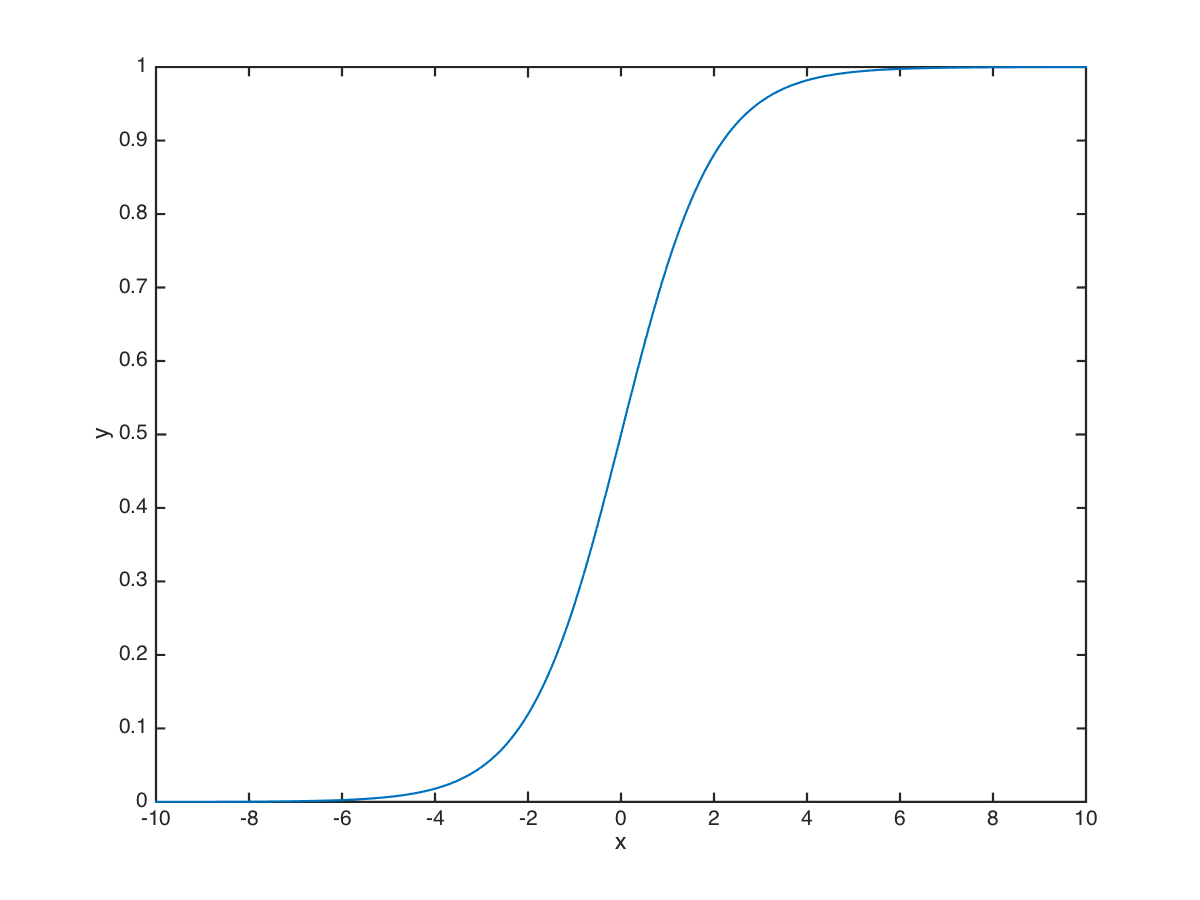
\includegraphics[scale=0.7]{sigmoid.png}
\caption{the Classical Sigmoid Function}
\end{center}
\end{figure}


It's obvious that the similarities of the features form the input vector of the features. The weights of the features form the weight vector for the input vector. As it is explained in the third chapter, the weight sum of the similarities of the features is computed and compared to the threshold. The sigmoid function should be shifted somehow to keep in accordance with the threshold. In order to do that, the input vector and the weight vector are extended by one dimension, $x'=\{1,x_1,x_2,...x_n\}$ and $w'=\{w_0,w_1,w_2,...w_n\}$. By using this method, the sigmoid function is shifted to the right by $-w_0$. For my approach, there are 10 features of  the inventor-patent instance. Therefore, there are 11 unknown parameters for the logistic regression including 10 weights and 1 threshold. The target of the logistic regression is to find the suitable values for the unknown parameters by using a dataset to do a training. After the training, each parameter will be assigned a value. If the parameter $w_i$ has a positive value, it means the input value $x_i$ has a positive correlation with the target value, in the contrary, the negative value implies a negative correlation. The larger is the absolute value of the parameter, the stronger is the correlation. As a machine learning algorithm, the overfitting problem should be taken care of. The overfitting problem is that after the training, although the model performs greatly well on the training data, the model has a bad performance for the new data. The overfitting problem is usually caused by the bad quality of the training dataset and the excessive training. In order to deal with the problem, some methods such as the regularization or stopping the training earlier can be used. After the training, the logistic regression can already helps us to distinguish the inventors. In addition, the conditional probability is unnecessary to compute. The weight sum of the similarities of the inventor-patent instances can be computed, compared to the threshold $-w_0$ and decide if the inventor-patent instances are matched or not.  
 
\subsection{the Training Data Generation}
The logistic regression in my approach is a binary classification. The inventor-patent instances from the inventor-patent instance database have IDs as the identification information. As it's explained before, the logistic regression training dataset is transformed from the inventor-patent instance dataset. The training data set is consist of the pairs of the inventor-patent instances. The features of the inventor-patent instances are used to compute the similarities for them. The identification information of the inventor-patent instances is used for the assignment of the classification label. Therefore, a binary label is assigned to each pair, "1" implies two instances matches and "0" implies they are not matched. The matching of the instances means that the inventor-patent instances have the same identification information, while the non-matching means that they have different identification information. The value assignment for weights is related to the similarity property. Because the similarity shows a great value when the instances are from the same persons, this assignment will give us positive values for the weights. Based on the features of the inventor-patent instances, the training data contains 10 dimensions for the 10 feature similarities. The following table shows two inventor-patent instances without text features and how to transform them into a piece of the training data.

\begin{table}[htb]
\scriptsize
\begin{center}
\begin{tabular}{ | c | c | c | c | c | c | c | c | c |}
\hline
ID & FirstName & LastName & Assignee & Tech Class & Lat & Lng & Country & Co-inventor \\ \hline
14398723 &PETER V & BOESEN & null &  381 & 41.58 & -93.64 & US & null \\ \hline
62514367 &WADE J& DOLL& CRAY INC & 439 &  47.65 & -122.40 & US & KELLEY DOUGLAS P \\
\hline
\end{tabular}
\end{center}
\caption{Examples of two Inventor-patent Instances except the Texts}
\end{table}
The "Tech Class" means the technology class and these two inventor-patent instances don't have sub-classes. The "Lat" means latitude. The "Lng" means longitude. Compute the similarities of the two inventor-patent instances based on all the features and transform the two inventor-patent instances into a piece of the training data as the following form. 

\begin{table}[htb]
\scriptsize
\begin{center}
\begin{tabular}{ | c | c | c | c | c | c | c | c | c |}
\hline
  Label  & First Name & Last Name & Assignee & Tech Class & Location & Co-inventor \\ \hline
   0 &0.2 & 0.167 & 0 &  0 & 0.2 & 0 \\ 
   \hline
\end{tabular}
\end{center} 
\caption{the Training Data Example}
\end{table}
The table above shows the transformed training data example. Because the two inventor-patent instances contain two different IDs, so the binary label is "0". The other columns show the similarities based on the names, the assignee, the technology class, the location and the co-inventors. The logistic regression is a supervised learning algorithm, so the training dataset for the logistic regression should contain the target value and multi-dimension data. The label of the transformed data is used as the target value and the rest of the data is used as the multi-dimension data as the inputs of the logistic regression. \\
Before the beginning of  training of the logistic regression, a subset of the inventor-patent instance dataset is selected as the training dataset. The transformation of the training dataset is applied. The transformed dataset which contains binary labels is used as the final training dataset. However, the training dataset size is large, because all the pairs of the inventor-patent instances are generated. If the subset of the inventor-patent instance dataset contains $n$ instances, then the transformed training dataset contains $\frac{n \cdot (n-1)}{2} $ pieces of the training data. For example, if there are 10,000 inventor-patent instances, there would be 49,995,000 pieces of the training data. The large training dataset may take a lot of time to be trained by the logistic regression. There are three possible solutions for that, the first solution is using the sampling method to generate a small dataset for training. The sampling method should be chosen carefully and the sampled dataset should be representative. However, the small training dataset usually cause overfitting problem. For example, a bad sampling method may choose a training dataset with a lot of outlines in it. The second solution is the optimization of the training method for a large-scale training. The optimization aims at speeding up the training process. The third method is to use some high-performance techniques  such as the distributed computing. 

\subsection{the Gradient Descent Method}
After generating the training dataset, the logistic regression is used as the training model to find the suitable weights and threshold. Like other machine learning algorithms, the logistic regression has a cost function, the cost function is  a negative logarithm form function.
\begin{equation}
J(\textbf{w})= - \frac{1}{m}[\sum_{i=1}^m ((y^{(i)}\log h_\textbf{w}(\textbf{x}^{(i)}) +(1-y^{(i)})\log (1-h_\textbf{w}(\textbf{x}^{(i)}))]
\end{equation}
\begin{equation}
h_\textbf{w}(\textbf{x})= \frac{1}{1+e^{- \textbf{x} \cdot \textbf{w}^T}}
\end{equation}
Here, $\textbf{x}^{i}$ means the ith piece of the training data in the training data set. $m$ is the training dataset size. $\frac{1}{m}$ is used to perform the normalization of the cost function. The cost function is a negative logarithm cost. The logistic regression training aims at minimizing this cost function by assigning each element in vector $\textbf{w}$ a suitable value. The method to compute the parameters by setting all the derivatives with respect to each parameter to zero is proved not analytic. An iterative method based on the gradient is usually used for the training of the logistic regression.
\begin{center}
\begin{figure}
\centering
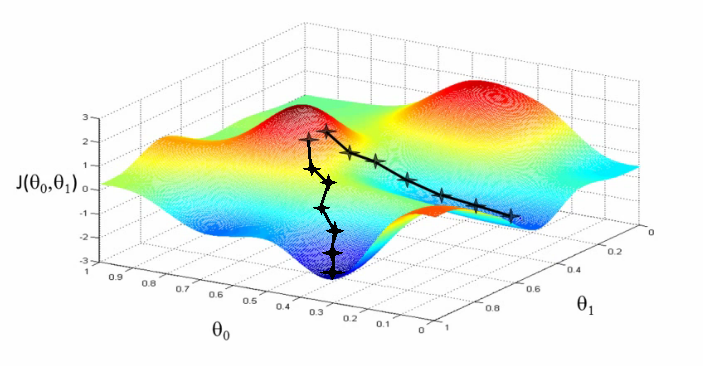
\includegraphics[scale=0.8]{gradient-descent.png}
\caption{the Gradient Descent Example \cite{gradient-descent} }
\end{figure}
\end{center}
The basic idea of the gradient descent training is to start at some point and use the gradients of the cost function to update the parameters until the cost function value reaches its local minimum. The figure 4.3 shows an example of the gradient-descent training with two parameters. At first, some initial values are assigned to the parameters. The gradients of parameters form a gradient vector pointed to a local minimum point of the cost function. Based on the gradient vector, update the parameter values iteratively until a local minimum is reached. The cost function gradient of the logistic regression with respect to a parameter is the following:
\begin{equation}
\frac{\partial J(\textbf{w})}{\partial w_i} =  \frac{1}{m} \sum_{i=1}^m (h_{\textbf{w}} (\textbf{x}^{(i)})-y^{(i)}) \cdot \textbf{x}^{i}
\end{equation}
Then a update of each parameter based on the gradient with respect to each parameter is performed.
\begin{equation}
w_i^{t+1}= w_i^{t} - \frac{\alpha}{m} \sum_{i=1}^m (h_{\textbf{w}} (\textbf{x}^{(i)})-y^{(i)}) \cdot \textbf{x}^{i}
\end{equation}
The $t$ represents the iteration number of the training process. The $\alpha$ represents the learning rate of the training which are also called the step size. The learning rate decides how much to update the parameter. The training process  keeps updating the parameters until the cost function reaches the local minimum point.  Although the gradient descent is an efficient method to train the logistic regression, it also has some disadvantages. First, the gradient descent method cannot promise to find the global minimum point. As it's shown in the figure 4.3, the cost function is not convex, so different initial values result in two different local minimum points. The cost function (equation 4.6) has been proved convex. The local minimum is necessarily the global minimum. The starting point decides how far away from the global minimum. The learning rate as a step size decides how long it takes to reach the global minimum. In addition, different values chosen for the learning rate  affect the behaviour to reach the global minimum or result in a failure for the training. The figure 4.4 shows the effects of the different learning rates on the training.
\begin{figure}
\centering
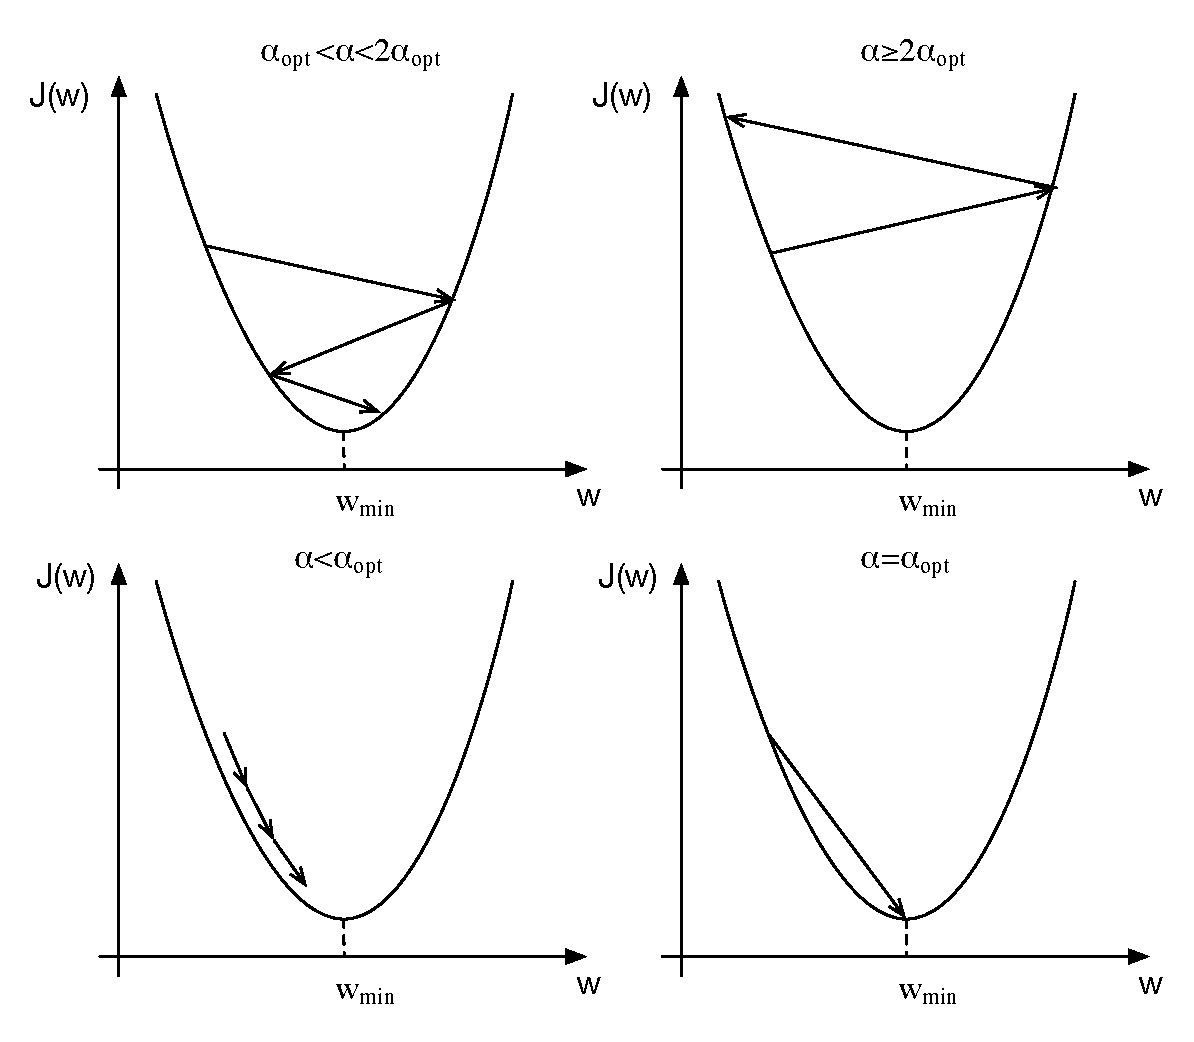
\includegraphics[scale=0.6]{learningRate.pdf}
\caption{the Learning Rate Effect}
\end{figure}
From the figure, there exists a perfect value $\alpha_{opt}$ for the learning rate. With the perfect value $\alpha_{opt}$, the cost function would reach the global minimum in one step. If 
 the learning rate is less than the $\alpha_{opt}$, the cost function will reach its global minimum step by step. The smaller is the size of the learning rate, the more steps would be needed to reach the global minimum. If the learning rate is larger than $\alpha_{opt}$ and less than $2\alpha_{opt}$, the cost function would oscillate around the global minimum. If the learning rate is larger than $2\alpha_{opt}$, the cost function goes away from this global minimum. The learning rate has a big effect on the training process. An alternative method for the training is the Newton-Raphson method which used the Hessian matrix instead of the learning rate.
The weight update of the Newton-Raphson method is to use the following formula
\begin{equation}
{\textbf{w}}^{t+1}={\textbf{w}}^{t}-{\textbf{H}}^{-1} \nabla {\textbf{w}} J(\textbf{w})
\end{equation}
\begin{equation}
\textbf{H}_{ij} = \frac{\partial^2 J(\textbf{w})}{\partial w_i \partial w_j} 
\end{equation}
The $\textbf{H}$ is the Hessian matrix. The Hessian matrix method uses the second order derivative instead of the learning rate. So it  uses less iterations to reach the global minimum. But for each iteration, the Hessian matrix and the inverse of the matrix  are computed and it would take longer time for one iteration and the Hessian matrix must be positive definite. For my approach, the learning rate method is applied. 

%Every machine learning algorithm faces the overfitting problem. The overfitting problem is the machine learning model fit the training data too much, and the model has bad performance for the new data. The figure 4.5 shows a overfitting training process. Usually to test if the model is overfitting, a training dataset is used for training and a test dataset is used for testing. Then keep track of the training dataset error and the testing dataset error. In the figure, when in the iteration t, the testing dataset error reaches its global minimum. After the iteration t, the testing dataset error begin to increase while the training dataset error keep decreasing. There are two popular techniques used to avoid the overfitting problem.  First technique is the regularization by adding a regularization term $\lambda R(\textbf{w})$ in the cost function. The Lasso regularization ($R(\textbf{w})=\vert \textbf{w} \vert$) and the Ridge regularization ($R(\textbf{w})=\sum_i w_i^2)$) are the most popular regularization methods. The $\lambda$ controls the importance of the regularization term. The value of $\lambda$ is based on the training dataset. If the training dataset is small or has a lot of outlines, the importance of the regularization should be large otherwise it should have a small value. As a hyper-parameter, there doesn't exist an efficient method to compute the regularization parameter. The regularization parameter is usually  adjusted manually by using the cross validation. Another popular technique to avoid overfitting is the "Stop-ealry" technique. This technique is just to stop the training before the overfitting. Before the training, the whole dataset  is divided into training dataset and validation dataset, usually the validation dataset is one third of the whole dataset. The validation dataset and the training dataset should not share any data.  During the training, the error of the validation dataset and the error of the training dataset are kept track of. When the validation dataset error reach the minimum or begin to increase, the training would be stopped. Compared to the regularization technique, the "Stop-Early" technique is easy to be implemented and has no hyper-parameter to be adjusted. So for my approach the "Stop-Early" technique is applied.


\section{Clustering Algorithms}
My approach combines the clustering algorithms with the logistic regression. After the training of the logistic regression, the logistic regression can identify two inventor-patent instances if they have the same inventor. However, as we know, many inventors cover several fields, sometimes change the location or change the assignee. Some inventor-patent instances from the same inventor have no similarities except the names of the inventors. Sometimes, these inventor-patent instances are considered from different inventors by using the logistic regression model. The clustering algorithm aims at helping to solve this problem by adding a transitive property for the identity of the inventor-patent instances to increase the accuracy of the inventor identification process. The clustering algorithm usually needs some distance function or similarity function to calculate the similarities between different objects. If the objects is multi-dimension data, the importance of the dimension is difficult to measure. As it's mentioned before, the clustering algorithm uses the results of the logistic regression. The weights are used to calculate the global similarities, the threshold is used for the assignment of the pre-defined parameters of the clustering method. In this section, the transitivity is first to be explained, then two clustering algorithms and how to use the threshold to set the pre-defined parameters are also introduced and how to apply the transitivity for the inventor identity is also described.

\subsection{the Transitivity}
As it's explained, the logistic regression sometimes considers two inventor-patent instances from the same inventor are from different inventors. The reason of the misclassification is not caused by the logistic regression itself. There are two possible reasons for the misclassification. The first reason is that the inventor may cover several fields. A database expert may also be good at the data mining. His patents may have different assignees, technology classes and text similarities. The second reason is that the inventor may change the location or the fields. Based on the two reasons, some inventor-patent instances of the same inventor only have the similar names of the inventors and small values of other similarities based on other features. In order to solve the problem, a transitivity property for the inventor identity is used to identify the inventor-patent instances. The figure 4.5 shows how to use the transitivity. 
\begin{figure}
\begin{center}
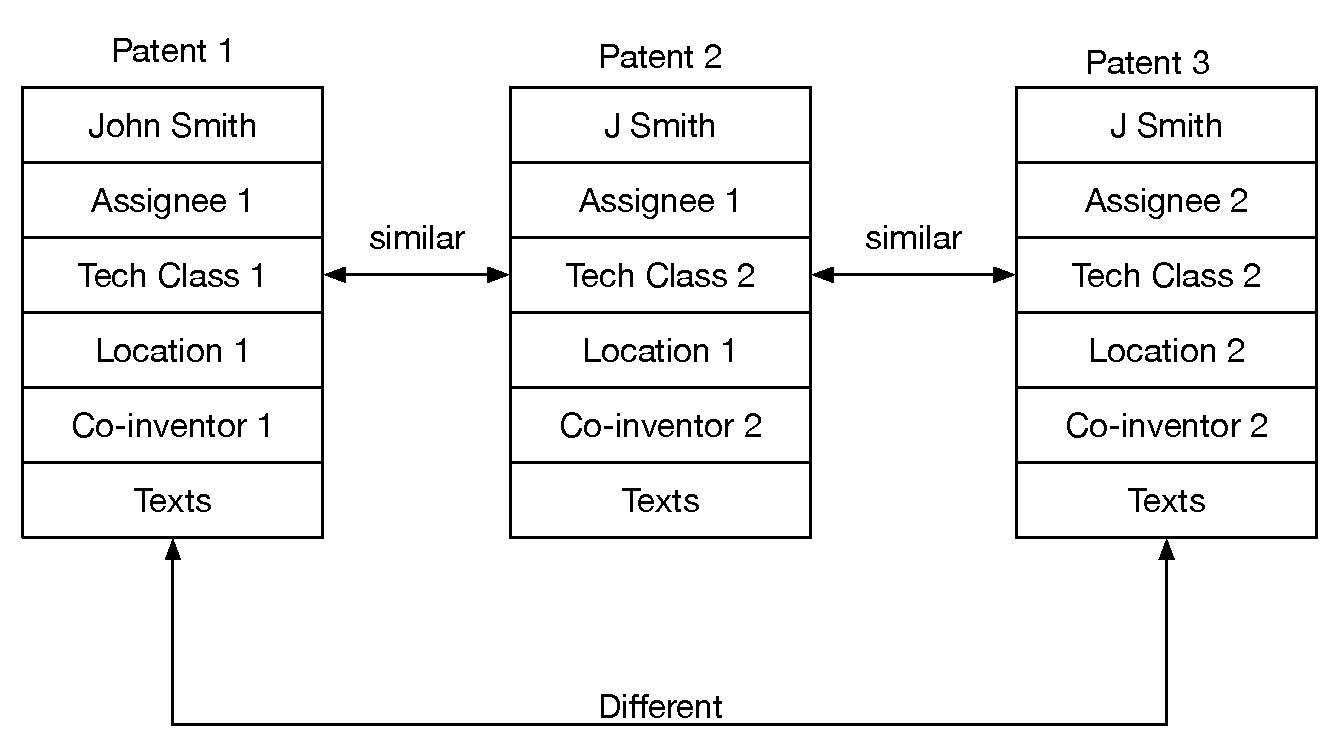
\includegraphics[scale=0.7]{Transitivity.pdf}
\caption{the Transitivity}
\end{center}
\end{figure}
The inventor-patent instance 1 and the inventor-patent instance 3 have different technology classes, assignees and locations. Even the inventor names of the two inventor-patent instances use different forms. The logistic regression model considers they are from two different inventors. But based on an assumption that the inventor may not change everything suddenly, so if the inventor-patent instance 2 can be found to have the same inventor as the inventor-patent instance 3 and the inventor-patent instance 1, then the inventor-patent instance 1 and the inventor-patent instance 3 are also considered to have the same inventor \footnote{The global similarities between the inventor-patent instance 1 and the inventor-patent instance 2 and the global similarity between the inventor-patent instance 3 and the inventor-instance 2 are both larger than the threshold}. However, the transitivity can also make some errors by making some different inventors as the same person. So a mechanism should be found to control the transitivity. The clustering algorithm is a good choice for this task. For my approach, the clustering method groups all the inventor-patent instances from the same inventors. In the following two sections, two clustering algorithms are introduced and how to use the clustering to implement the transitivity is also explained.

\subsection{the Agglomerative Hierarchical Clustering}
The agglomerative hierarchical clustering is a classical clustering. The basic idea of the hierarchical clustering is to merge successively the clusters of the objects until all the objects are in  one cluster. The figure 4.6 shows an example of the hierarchical clustering. 
\begin{figure}
\centering
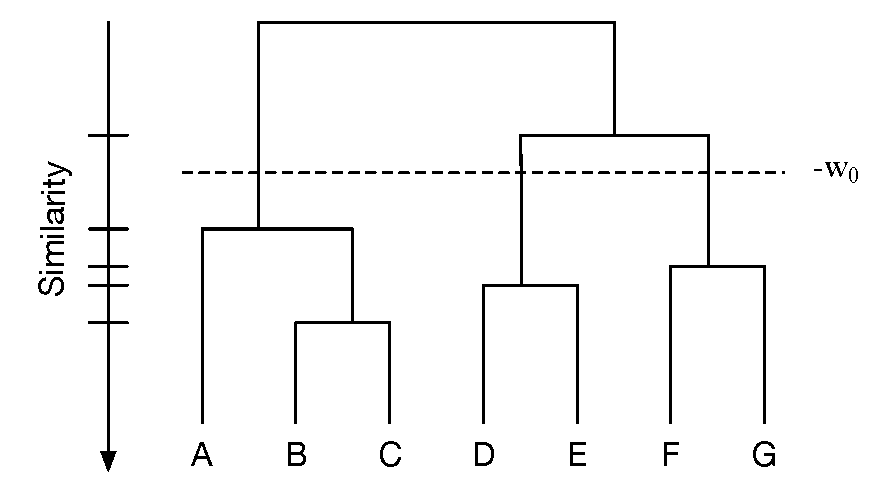
\includegraphics[scale=0.5]{Hierarchical.pdf}
\caption{the Hierarchical Clustering Example}
\end{figure}
Every object is first put into a single cluster. For each iteration, the similarities between all pairs of the clusters are computed. The two clusters with the best similarity is merged. Keep doing that until all the objects are in the same cluster. The objects in our approach is the inventor-patent instances while the similarity measure is the global similarity as a weight sum of all the feature similarities. However, for our approach, the target of the clustering algorithm is to put all the inventor-patent instances of the same inventors into the same clusters. It is not necessary to keep the hierarchical clustering running until only one cluster is left. The clustering process should be stopped based on a suitable criteria. The dashed line in the figure 4.6 represents where to stop the agglomerative hierarchical clustering. The stop criteria for the hierarchical clustering is the threshold from the logistic regression training result. If in a certain iteration, the best similarity of the clusters is less than the threshold, which means the inventor-patent instance clusters have a small probability from the same inventor, then the clustering method is stopped.  The algorithm 1 shows the persudo codes for agglomerative hierarchical clustering for my approach. \newline

\begin{algorithm}[b]
\caption{the Agglomerative Hierarchical Clustering}
\begin{algorithmic}
\REQUIRE
	 a set of inventor-patent instances $\textbf{X}=\{x_1,x_2,...,x_n\}$
\ENSURE
	 a set of clusters $\textbf{C}=\{c_1,c_2,...,c_m\}$
\FOR{ $i=1$ to $n$}
          \STATE $c_i=\{ x_i \}$
\ENDFOR	

\WHILE{$(C.size>1)$} 
\STATE  ($C_{i},C_{j}$)= maximum sim($c_i,c_j$) for all $c_i$, $c_j$ in $\textbf{C}$
\STATE  $maxSim=sim(C_{i},C_{j})$ 
 \IF  {$maxSim<\theta$} 
\STATE break;
\ENDIF
\STATE remove $C_{i}$,$C_{j}$ from   $\textbf{C}$
\STATE add ({$C_{i}$,$C_{j}$}) in  $\textbf{C}$
\ENDWHILE

  

\end{algorithmic}
\end{algorithm}


The transitivity of the inventor identity is controlled by the methods to calculate the cluster similarity. The methods of the cluster similarity calculation  affects which clusters will be merged.
There are three methods for the cluster similarity calculation. 
\begin{itemize}
\item \textbf{Single Linkage Clustering:}
The single linkage clustering computes the similarity between clusters by using the best similarity between any pairs of the objects from the clusters. For each iteration, the clusters whose most similar object pair has the highest similarity is merged. The single linkage clustering can be implemented in an very efficient way. Compute the similarities of all the pairs and sort the pairs based on the similarity. Pick the pair of the objects in order and merge the clusters if the   two objects belong to different clusters. 
\item \textbf{Group-average Linkage Clustering:}
The group-average linkage clustering compute the average similarity between objects from two clusters. Usually the group-average linkage clustering method is slower than the single linkage clustering, but it's more robust. The average similarity between two clusters could be approximated by using the mean object of the clusters if it's computable. The quality of the approximation is based on the data structure of the objects. If the mean object works well, the time complexity can be reduced to $O(n^2)$.
\item \textbf{Complete Linkage Clustering:}
The complete linkage clustering computes the similarity of the clusters by using the worst similarity between the pairs of the objects from the two clusters. The complete linkage clustering is the slowest among these techniques. The time complexity is $O(n^3)$.
\end{itemize}

Three different types of clustering methods offer three different transitivity levels for the clustering. The single linkage clustering offers the strongest transitivity. Because the threshold is used as the stop criterion. The single linkage clustering can be considered as that if there is a pair of objects from two clusters whose similarity is larger than the threshold, they will be merged somehow in the end. From a different perspective, the mechanism encourages the similarity transitivity. So if A is similar to B and B is similar to C, A is similar to C. This property is also called the chain rule. The complete linkage clustering avoids the transitivity. Because it uses the worst similarity, the similarity between the pairs of objects in the cluster should be larger than the threshold and it means that the objects in the same cluster should be similar to each other. The transitivity of the group-average linkage clustering is stronger than that of the complete linkage clustering and weaker than  that of the single linkage clustering. \newline

As it is explained before, the hierarchical clustering with different cluster similarity calculation methods provides three different transitivity levels. However, it is not flexible because the transitivity only has three levels, the complete transitivity for the single linkage clustering, no transitivity for the complete linkage clustering and the transitivity between them for the group-average linkage clustering. Compared to the hierarchical clustering, the density-based clustering can provide a more flexible method to control the transitivity. 
\begin{figure}
\centering
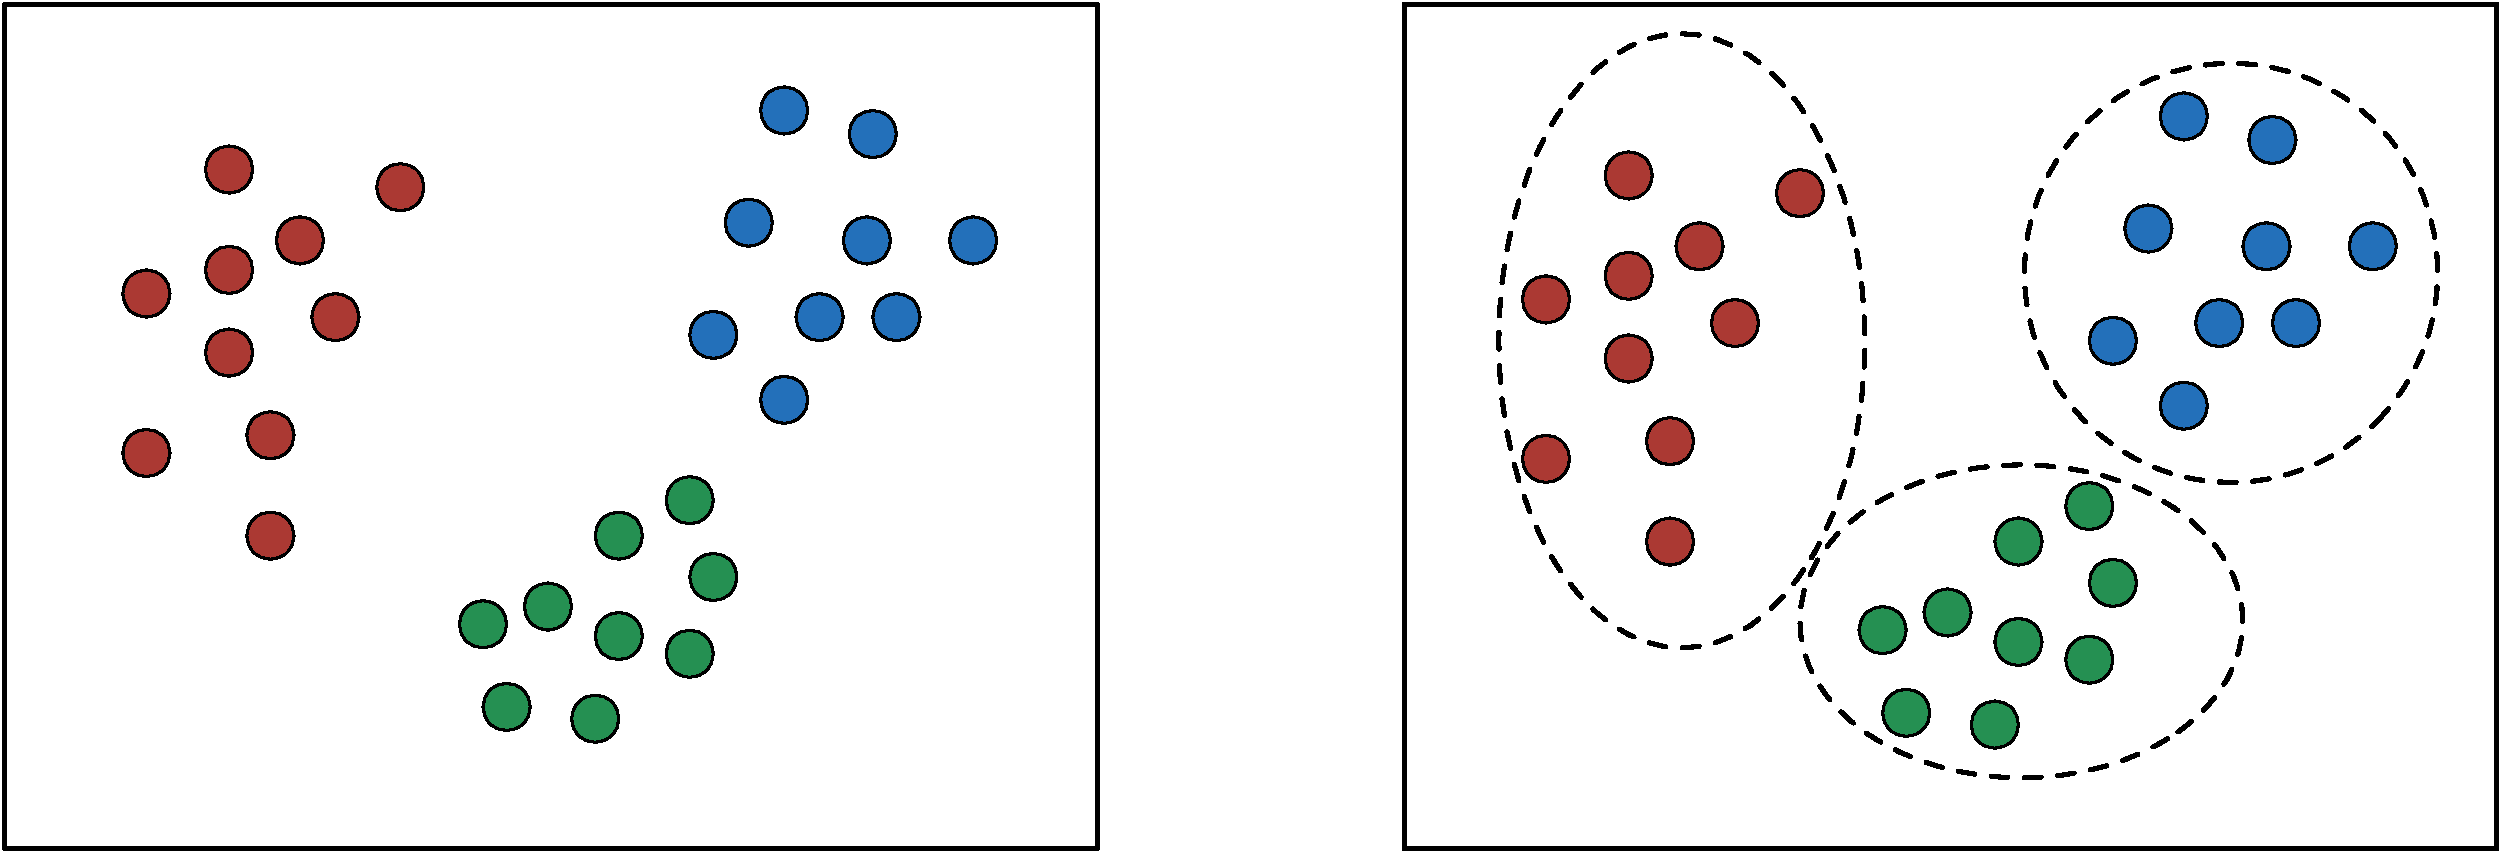
\includegraphics[scale=0.3]{density-basedClustering.pdf}
\caption{the Density-based Clustering Example}
\end{figure}



\subsection{the Density-based Spatial Clustering of Applications with Noise}

The DBSCAN is a density-based clustering. Put every objects in the multi-dimensions feature space and measure the distance between the objects based on a distance function. As it is shown in the figure 4.8. Some regions contain a lot of objects and some don't. Based on the density of the region, the dense regions are considered as the clusters which are separated by the sparse regions. In order to apply this clustering, a local density of a point should be defined. The local density is represented as the neighbours of the points.
\begin{equation}
N_\theta(q)=\{p \in D| distance(p,q) \le \theta\}
\end{equation}
Here, $\theta$ represents the largest distance between the neighbours and the point $q$. $distance(p,q)$ represents the distance between p and q. If the number of the neighbours of an object is larger than a pre-defined number, the object is  considered as a core object. The pre-defined number is called minimum points (MinPts).  In order to apply the DBSCAN, there are some concepts which should be defined first.
\begin{figure}
\centering
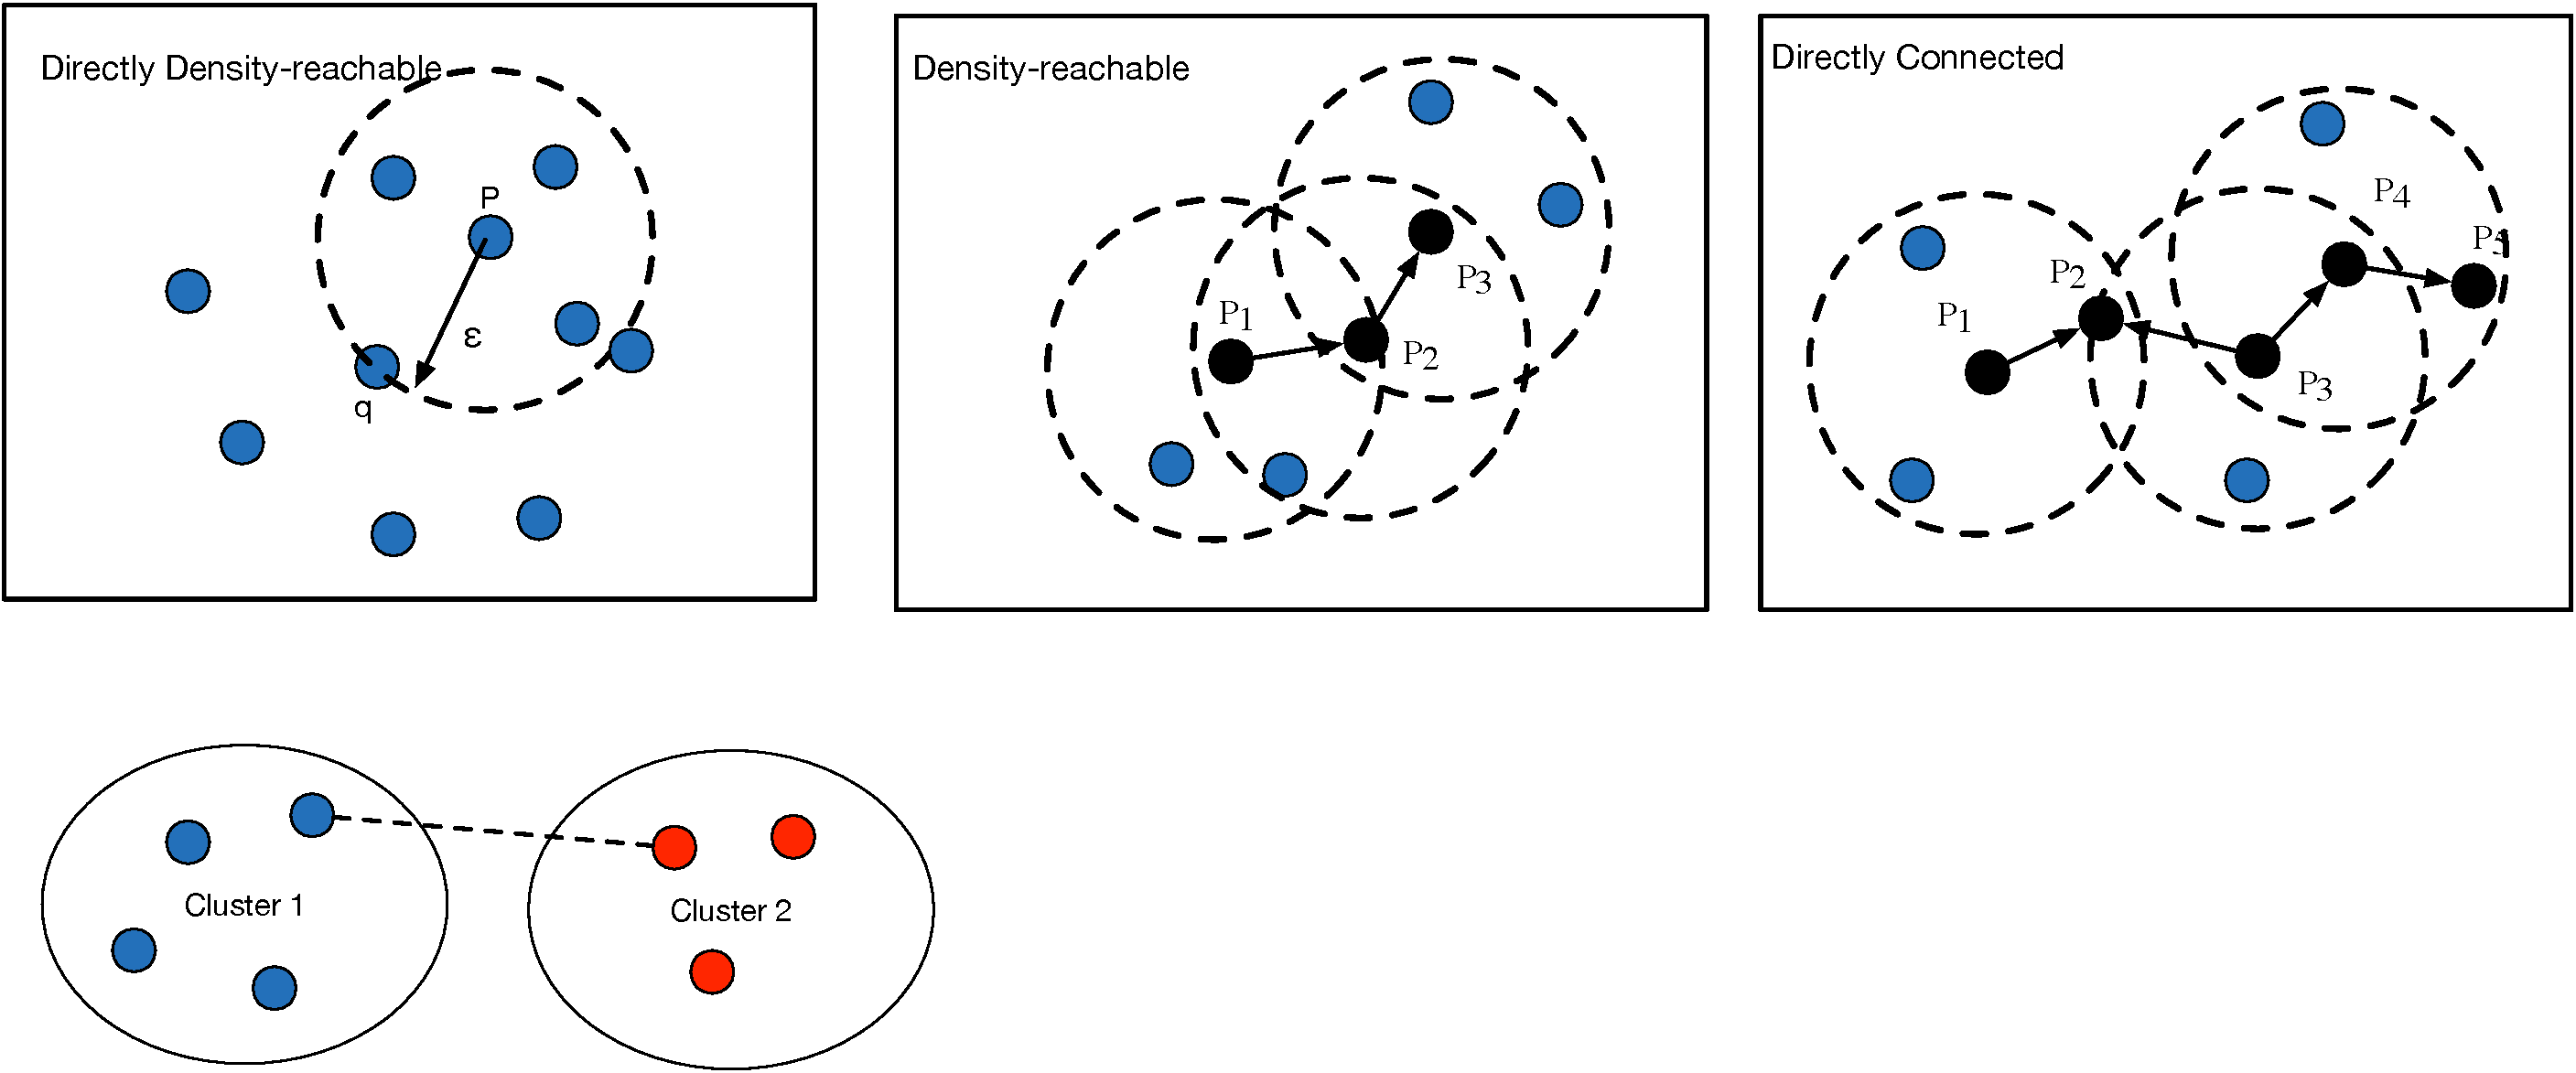
\includegraphics[scale=0.4]{DBSCANPre.pdf}
\caption{the Basic Definition for the DBSCAN}
\end{figure}
\begin{itemize}
\item \textbf{Directly Density Reachable}:  As it's shown in the figure 4.9(a), if p is a core object and the distance between p and q is less than or equal to the $\theta$, q is called directly reachable from p.  
\item \textbf{Density Reachable}: As it's shown in figure 4.9(b), if the $P_2$ is density reachable form $P_1$ and $P_3$ is density reachable from $P_2$, then $P_3$ is density reachable from $P_1$.  
\item \textbf{Density Connected}: If two objects are density reachable from at least one same core object, then the two objects are density connected. As it's shown in figure 4.9(c), $P_2$ is density reachable from $P_1$ and $P_3$, but $P_1$ and $P_3$ are not density connected as $P_2$ is not a core object. $P_3$ and $P_5$ are density connected because they are density reachable from the same core object $P_4$.
\end{itemize}

After the definition of these basic concepts, the cluster of DBSCAN can be described based on these concepts. 
\begin{itemize}
\item \textbf{Cluster}: the subset of a dataset which is satisfied by the maximality and the connectivity.
\begin{itemize}
\item \emph{Maximality}:  The objects which are not in the cluster should not be density reachable to any object in the cluster.
\item \emph{Connectivity}: Any two objects in the cluster should be density connected to each other.
\end{itemize}
\item \textbf{Noise}: The objects which don't belong to any cluster is called noise.
\end{itemize}
The DBSCAN is trying to build these clusters by successively finding all density reachable objects of the core objects and assign the core objects with their density reachable objects to clusters. The pseudo code of the DBSCAN is described as follows:
\begin{algorithm}
\caption{DBSCAN}
\begin{algorithmic}
\FOR{each object $o \in Dataset$}
\IF {$o$ is not visited and $o$  is a core object} 
\STATE Collect all the objects which are density reachable from $o$. Assign them to a cluster.
\newline Mark all the objects and $o$ as visited objects
\ELSE
\STATE Assign $o$ to noise and mark $o$ as the visited objects
\ENDIF
\ENDFOR
\end{algorithmic}
\end{algorithm}

The classical DBSCAN usually uses the distance function to measure the difference of two objects. For my approach, the similarity function is used instead of the distance function. The neighbours of the inventor-patent instance $o$ are the instances which have a similarity larger than a specified value with $o$. The threshold generated by the logistic regression is used as the specified value here. Because a similarity larger than a threshold implies the two inventor-patent instances are from the same person, it's obvious that the inventor-patent instances from the same person are neighbours of each other. In fact, the DBSCAN uses a transitivity to collect all the objects and assign them to the same cluster. The transitivity is described by the density connect concept. As it's defined above, the two objects are density connected if they are density reachable from a core object. The core object is used to connect objects and the core object is defined by the number of the MinPts.  
Therefore, the MinPts is used to control the transitivity of DBSCAN. For my approach, the neighbours of a object don't contain itself. So if the MinPts is set to 1, the DBSCAN considers all the inventor-patent instances which have at least one similar inventor-patent instance as the core objects. The DBSCAN with the MinPts as 1 works the same as the single-linkage clustering which gives the largest transitivity. Increasing the value of the MinPts  decreases the identity transitivity. When the MinPts is larger than a value, there will be no core objects and all the objects in the dataset are considered as noise. The noise is separately put into clusters. However, the control of the inventor identity transitivity of DBSCAN is much more flexible compared to the hierarchical clustering because of the MinPts is a parameter which can be adjusted.  

\section{the Patent-publication Matching}
As it's explained before, the publication database sometimes can provide some identification information of the author and the identification information is not always available. The patent-publication matching is used for improving the clustering result. In this section, three different methods to do the patent-publication matching are introduced. 

\begin{itemize}

\item \textbf{Non-patent Reference(NPR) Matching}:
In the patent document, there is a reference list. The list contains the references of the patent. The references of the patents can be divided into two categories: the patent reference and the non-patent reference. The patent references refer to some other patent documents while the non-patent references refer to some documents other than the patent documents. Usually it contains some publications, if some publications contain the same name of the inventors. It has a big probability that the inventor owns the publication, because the inventors are likely to cite his own publications. The first method to do the matching is called the non-patent reference matching. We first extract all the publications by doing a query in the publication database with the inventor's name. Check the patents' non-patent references in the patent document in the inventor-patent instance cluster to see if the publications' titles have appeared in the non-patent references. If so, the author is matched to the cluster. Choose the author which has been matched the most times and assign the author ID to the cluster.

\item \textbf{Assignee-affiliation Matching}:
Each patent has an assignee and each publication has an affiliation. Sometimes the inventor's patent assignee and publication affiliation are the same organization. So the assignee-affiliation matching tries to match the patent and the publication by comparing the patent assignee name and the publication affiliation name. If they are  same, the cluster of the patent will be assigned the author ID with the most matching times.

\item \textbf{Abstract Matching}:
The text mining technique can also be used to match the patent and the publication. The abstract of the publication is usually provided by the publication database. So the abstract of the patent and the abstract of the publication can be used to calculate a text similarity. The normalized term frequencies are calculated for the abstract of the publication and the abstract of the patent. The cosine similarity is used to measure the similarity of the patent abstract and the publication abstract. For each patent, choose the publication with the best text similarity as the matching publication. In the same way, assign the publication author ID to the inventor-patent instance cluster and choose the ID which has been matched most. 
 
\end{itemize}

The three methods of the matching should be done in a serial order, the NPR matching, the assignee-affiliation matching and the abstract matching. Three matching methods could not guarantee the absolutely correct matching. The serial order is based on the probability of the matching method for correctly matching. For my thesis approach, the NPR matching is considered as the most trusted method compared to the other two methods. Because the assignees and affiliations as the organizations and institutions, they usually contains a big staff. Taken the non-unique forms of the inventor names into consideration,  the assignee-affiliation matching is not as reliable as the NPR matching. The text similarities are always larger than 0 and the publication with the best similarity should always be chosen if the abstract of some publications are provided.\newline

In addition, the patent-publication matching is performed after the clustering. For each cluster, the inventor name which appears most in the cluster is used as a keyword to do a query in a publication database. The result of the query contains a set of the publications. The three methods of the patent-publication matching are performed in a serial order to assign an ID to each inventor-patent instance cluster if possible. Then check all the clusters which have IDs, if some clusters have the same IDs, they are merged.

\section{Practical Issues}
In this section, some practical issues of the implementation of the approach are introduced. These issues include some techniques for the efficiency, the value selection for some parameters and the patent-publication matching problem.

\subsection{the Latent Semantic Indexing(LSI)}
As it's mentioned before, the normalized term frequency vector is used to represent the texts of the patent such as the abstract, the claim, the description and the title. The length of the normalized term frequency vector is the number of the different stems of the text. As the size of the text increases, the length of the vector increases as there are more stems in the text. The large size of the vector increases the time of text similarity computation. There are two methods used for my approach to decrease the dimension of  the normalized term frequency vectors. Fall, Torcsvari, Benzineb, and Karetka (2003) shows that  using only the first 300
words from the abstract, the claim, and the description, the performance is better than those using the full texts regardless of which classifiers are used \cite{tseng2007text}. For my approach, the first 300 words of the abstract, the claim and the description are used instead of the full text. For the convenience of the computation, usually a normalized term frequency matrix are built for the text dataset. The rows are usually related to the stems of all the texts. The columns are related to the special indexes of the texts. As the size of the text dataset increases, the number of the rows  also increases.  A technique called Latent Semantic Indexing (LSI) by using the singular value decomposition is used to do the dimension reduction. The basic idea is based on the correlation of the stems of the texts. For example, "computer" and "science" usually appear together in the text. So a combination of these two words can be used instead of two words separately. Usually the matrix $\textbf{A}$ is a sparse matrix, because for each text, it only contains a small subset of the whole stem set. Because of the sparsity, $\textbf{A}^T \cdot \textbf{A}$ is a good approximation of the covariance matrix for the stems. Then the decomposition of the $\textbf{A}^T \cdot \textbf{A}$ can be applied.
\begin{equation}
\textbf{A}^T \cdot \textbf{A} = \textbf{U}  \Lambda \textbf{U}^{-1}
\end{equation}
$\textbf{U}$ contains all the eigenvectors and $\Lambda$ contains all the eigenvalues. The eigenvectors represent a new orthogonal basis system, while the eigenvalues represent the variances when the original vectors are projected to the new basis system. In order to do the dimension reduction, the first $n$ eigenvectors with the largest eigenvalues are chosen as the new basis system. The original vectors are projected to the new basis system. $n$ is usually from 300 to 400 \cite{ASTCA}. For my approach, 300 is chosen. 

\subsection{Initial Values}
The gradient descent is used for the training for the logistic regression. The final result is based on the learning rate and the initial values for the parameters $\textbf{w}^0$. Although the initial values are very important and decide how far away is from the global minimum point, there doesn't exists any criterion to choose the initial value for the parameters and choice of the initial values for the parameters are not critical. However, setting all the parameters to zero usually works fine \cite{allison2008convergence}. 

\subsection{the "Stop-early" Technique}
\begin{figure}
\centering
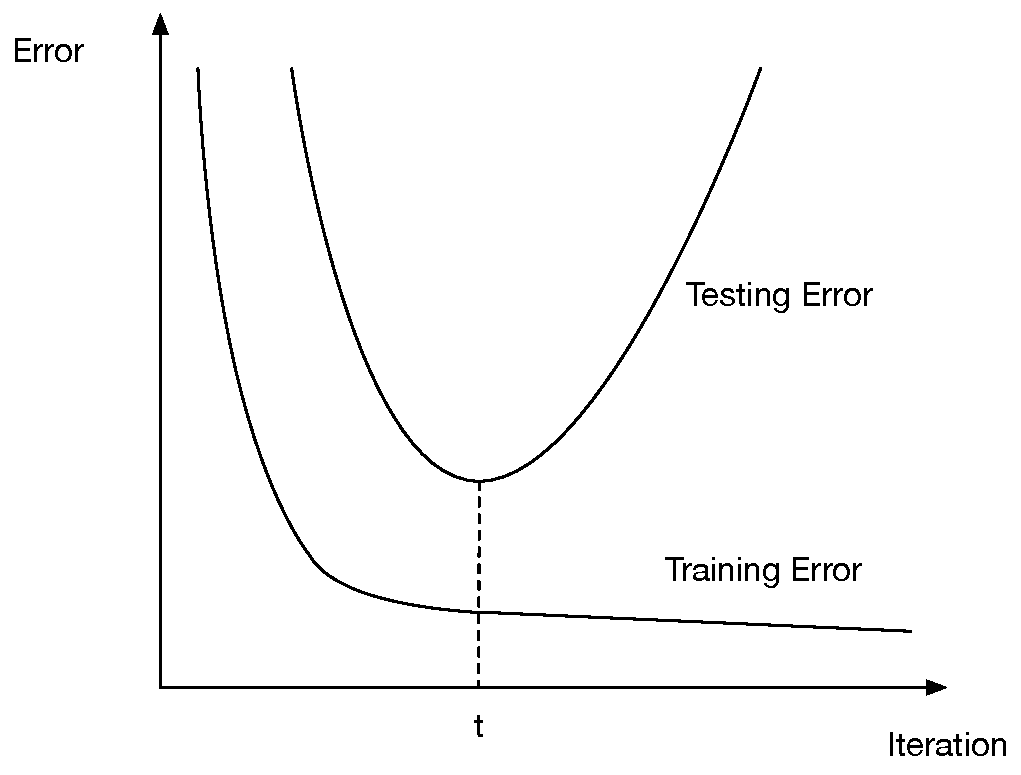
\includegraphics[scale=0.6]{overfittingExample.pdf}
\caption{the Overfitting Example}
\end{figure} 
Another problem for the logistic regression is the overfitting problem. The performance of the logistic model for the new data gets worse and worse after some point if the training process is kept going on. The figure 4.9 shows a overfitting training process. Usually to test if the model is overfitting, a training dataset is used for training and a test dataset is used for testing. Then keep track of the training dataset error and the testing dataset error. In the figure, when in the iteration t, the testing dataset error reaches its global minimum. After the iteration t, the testing dataset error begins to increase while the training dataset error keeps decreasing. There are two popular techniques for decreasing the overfitting effect, the regularization and the "Stop-early" technique. These two techniques aim at reducing the size of each parameter dimension. The regularization technique adds a regularization term to the cost function.
\begin{equation}
J(\textbf{w})= - \frac{1}{m}[\sum_{i=1}^m (y^{(i)}\log h_\textbf{w}(\textbf{x}^{(i)}) +(1-y^{(i)})\log (1-h_\textbf{w}(\textbf{x}^{(i)}))+\lambda R(\theta)]
\end{equation} 
Based on the form of the $R(\theta)$,  there are two popular methods for the regularization, Lasso regularization and Ringe regularization. The regularization needs a regularization parameter $\lambda$. In order to find a suitable value for $\lambda$, a lot of experiments should be taken and the value for $\lambda$ varies between different training datasets. Compared to the regularization method, the "Stop-early" method is easy to be implemented and not necessary to import a new parameter. The method divides the training data into two separate parts, the training dataset and the validation dataset. The training process only uses the training dataset for training. While the validation dataset is used to represent the new data, the average error of the training data and the average error of the validation dataset are kept track of during the training process. The batch gradient descent for the logistic regression  always decreases the cost function value and the average training dataset error. The average validation  dataset error as the new data  keeps decreasing until a certain point. When the validation error begins to increase, the training process is to be stopped. The values of the parameters from the last iteration are used as the final result.
 
\subsection{the Bold Driver Technique}
Another important parameter for the logistic regression is the learning rate. The learning rate used  for the logistic regression somehow decides what result will be found in the end and affects the training time. With a smaller learning rate, the training process takes a long time. But with a large value, the divergence problem may occur. Usually for the training, keeping a constant learning rate results in a long training time. The bold driver technique is a good method to adapt the learning rate during the training. The basic idea behind this technique is that if the current position is far away from the global minimum point, the learning rate should be large in order to reach the global minimum fast. If the position is near the global minimum point, the learning rate should be small in order not to go over the global minimum point. The method of the bold driver technique is to keep track of the average training dataset error during the training process. If the average training dataset error decreases, the learning rate should be multiplied by a factor $\alpha$ ($\alpha>1$). If the average training dataset error increases which means the global minimum point is skipped, the last update of the weights is to be cancelled. The learning rate is multiplied by another factor $\beta$ ($0<\beta<1$). The learning rate is to be kept decreasing until the training dataset error starts again to decrease. The learning rate sometimes tends to zero, because the current position is too close to the global minimum point. Therefore, if the learning rate is too small such as less than $10^{-10}$, the training process is also to be stopped. It has been shown that the adaptive learning rate works better than a fixed learning rate especially a much faster convergence. For my approach, the learning rate is to be given a small learning rate at first. The learning rate is adapted by the bold driver technique for each iteration, the chosen $\alpha$ and $\beta$ are $1.1$ and $0.5$. The performance of the training doesn't depend critically on these values. The chosen values take the heuristic guideline of the paper of Roberto Battiti \cite{battiti1989accelerated} as a reference.  

\subsection{Europe PMC}
For the patent-publication matching, a publication database should be used and it should provide author IDs. Europe PMC is a good publication database which provides a lot of useful information for the publication, including the author ID, the abstract and the affiliation. There are two drawbacks of the Europe PMC. The first one is that not all the publications contain the author ID, the publication abstract and the affiliation. The second  is that it uses the last name plus the first letters of the middle name and first name as the inventor name. The three patent-publication matching methods are not always available  because of the first drawback. In addition, a lot of irrelevant results are returned when a query is done. For example, if the inventor's name of a cluster is "John Smith". "Smith J"  is used as the keyword to do a query in the publication database. As a result, the publications of  "John Smith" and "Jack Smith" may both be returned. Although Europe PMC has drawbacks, it's the best publication database which I can found to help me to do the patent-publication matching. In order to do the patent-publication matching more efficiently, some changes for the patent-publication matching have been applied. First, after the clustering, each cluster is assigned an inventor name and the inventor name is transformed into the "last name+ first letters of the middle name and the first name" form. Choose the clusters with the same names as the candidates for the patent-publication matching. Second, if the three matching methods fail, the cluster is assigned a null ID. The clusters with  null IDs are not merged. If one of the matching methods successes and the author ID is not available, the publication ID is assigned to the cluster instead of the author ID.  

\section{"Invdenti" Java Project Description}
In this section, the details of the Java project for my approach are introduced. The big picture of the Java project is introduced first. Then the development environment, some data structures used for the java project and the configuration file are also introduced. In the end, the details of six core parts of the Java project are introduced. They are related to the text extractor, the preprocessing, the logistic regression, the clustering, the patent-publication matching and the evaluation.

\begin{figure}
\centering
\includegraphics[scale=0.5]{codeUML.pdf}
\caption{the Basic Structure of the Java Project}
\end{figure}


\subsection{the Basic Structure of the Java Project}
The figure 4.10 shows the big picture of my project. For convenience, I called the project "Invidenti" which represents the "Inventor Identification". The project is connected to two inventor-patent instance datasets. The first dataset is the Flemming's dataset and the second one is "E\&S" dataset. The Flemming's dataset is downloaded from the Flemming's website \footnote{Flemming's Database Download Link: \url{https://dataverse.harvard.edu/dataset.xhtml?persistentId=hdl:1902.1/15705}}. The E\&S dataset is created by using the CSV file provided by the USPTO. \footnote{E\&S Database Download Link: \url {http://www.patentsview.org/workshop/participants.html} } There are two APIs used by the project. One is the patent full-text search engine (Patft) API and the other is the Europe PMC API which have been introduced before. The first is used to extract the patent texts and the second is used for extracting the publication information. The project contains six core parts which is marked with bold font and rectangular shape. The first one is "Text Extractor". It's a web spider which uses the Patft. The web spider is designed specially for the patent document file returned from the API. It precisely extracts the title, the abstract, the claim and the description from the patent document. The extracted texts are stored into a number of text files. The second part is the preprocessing which is used to preprocess the patent texts.  From the figure, the texts and the data from the datasets are preprocessed before they flow into the clustering part and the logistic regression part. The third part is the logistic regression. The logistic regression part  is connected to two datasets and one text dataset. The text dataset is created by the text extractor. The two datasets are the Flemmimg's datasets and a subset of the E\&S dataset which is randomly chosen from the original E\&S dataset. The logistic regression is used to find suitable values for the threshold and the weights. These values are provided to the clustering part. The clustering part is also connected to two datasets and one text dataset. The only difference compared to the logistic regression is the E\&S dataset which is the data from the original E\&S dataset expect the data used for the logistic regression. The clustering part performs clustering algorithms and passes the clustering result to the patent-publication matching part. The patent-publication matching part uses the Europe PMC API and tries to refine the clustering result. The refined clustering result is passed to the evaluation part. After the evaluation part, the final clustering result and the performance result are generated.   

\subsection{the Development Environment and ToolKits}
This Java project is programmed in Java SE development Kit 8. The version of Java is 1.8.0\_43. The programming environment is intellij 15.0.3. Because there are many toolkits which can help the project to do the text mining, text extracting and etc, the Apache maven is used to help the project to manage the toolkits. The version of the maven is 3.3.3. The table 4.4 shows the main tookits used in the project and what they are used for.  

\begin{table}[b]
\centering

\begin{tabular}{|c|c|}
\hline
Toolkit name & Toolkit Role in the Project \\
\hline
carrot2 & Text Mining \\
\hline
jdbc  & "Sqlite" Database Library \\ 
\hline
webMagic & Text Extracting.\\
\hline
ini4J& Manage the configuration \\
\hline
log4j & Manage the format of the output \\
\hline
java-string-similarity & Compute the String Similarity \\
\hline
jblas, Apache math3 & Linear Algebra Libraries \\
\hline

\end{tabular}

\caption{the Toolkit Table}
\end{table}

The "carrot2" package is used to help the project to do the preprocessing for the texts. The "carrot2" is a good text clustering package but it only deals with the texts. So the "carrot2" clustering function is not used for the project. Because the Flemming's database is the sqlite format. In order to keep in accordance with this format, the database created by the approach is also  the sqlite format. The jdbc is a good sqlite java library which can read or write the database. WebMagic is a toolkit which can help the project to create the spiders to extract texts from the website. The toolkit is used to create two special spiders to extract the information of the patents and the publications. "Java-String-Similarity" toolkit can be used to calculate the string similarity based on different methods. "Jblas" and "Apache math3" are good linear algebra toolkits which help the project do some matrix computation for the latent semantic indexing and the logistic regression training. "Ini4J" is to help the project to manage the configuration while the "log4j" is to help the project manage the output of the project which can control the color, format of the output. 

\subsection{the Configuration File}
The configuration used for the project aims at controlling the behaviour of different parts and providing a lot of options to initialize the project. The configuration file used in the project is the "invidenti.ini". The table 4.5 shows the basic structure of the configuration file.
\begin{table}
\centering
\begin{tabular}{|c|c|}
\hline
\multicolumn{2}{|c|}{\textbf{Distance Options}} \\
\hline
Comparison Options & feature selection   \\
\hline
Options & the features' names \\
\hline
PCorrelation & switch between the distance function and the similarity function. \\
\hline
Weights & the weights for the features\\
\hline
\multicolumn{2}{|c|}{\textbf{Dataset}} \\
\hline
TrainingDataInputPath & the training dataset csv file path \\
\hline
TrainingDataOuputPath& the generated training database's storage path \\
\hline
InfoDataPath & the inventor-patent instance information database's storage path \\
\hline
TextPath & the patent document texts' storage path \\
\hline
SamplePath & the storage path for the training dataset and the testing dataset  \\
\hline
\end{tabular}
\caption{the Configuration Structure}
\end{table}
The configuration contains two parts. The first part is used to store the configuration of the distance function. The distance function in my approach is a general concept. It can be a distance function or a similarity function. The switch between them is controlled by a parameter called "pCorrelation". If "pCorrelation" is true, the distance function is transformed into a similarity function, otherwise it's a classical distance function. There are 10 parameters to control the feature selection. Each parameter is related to a feature. If the parameter is true, then the related feature will be used in the approach. There are another 10 parameters which is used to store the weights of the features. In fact, if the training is performed, these values will be used as the initial values for the training. If the training is not performed, these values will be used to create a general distance function.  There is another parameter which stores all the names of the features. The second part of the configuration file is for the datasets. The "TrainingDataInputPath" stores the path of the csv file of the training data. The csv file is used to create a database of the training data. The "TrainingDataOutputPath" is the location where the training database will be stored. The "infoPath" is the inventor-patent instance information database. This database for my approach is the Flemming's inventor-patent instance database. The "TextPath" is the location where the texts of the patents are stored. The "SamplePath" is the location where the training dataset and the testing dataset are stored. This path is used for the evaluation. The original training dataset will be divided into two parts, the training dataset for the training and the testing dataset for the performance evaluation. 

 

\subsection{the Text Extractor}
\begin{figure}
\centering
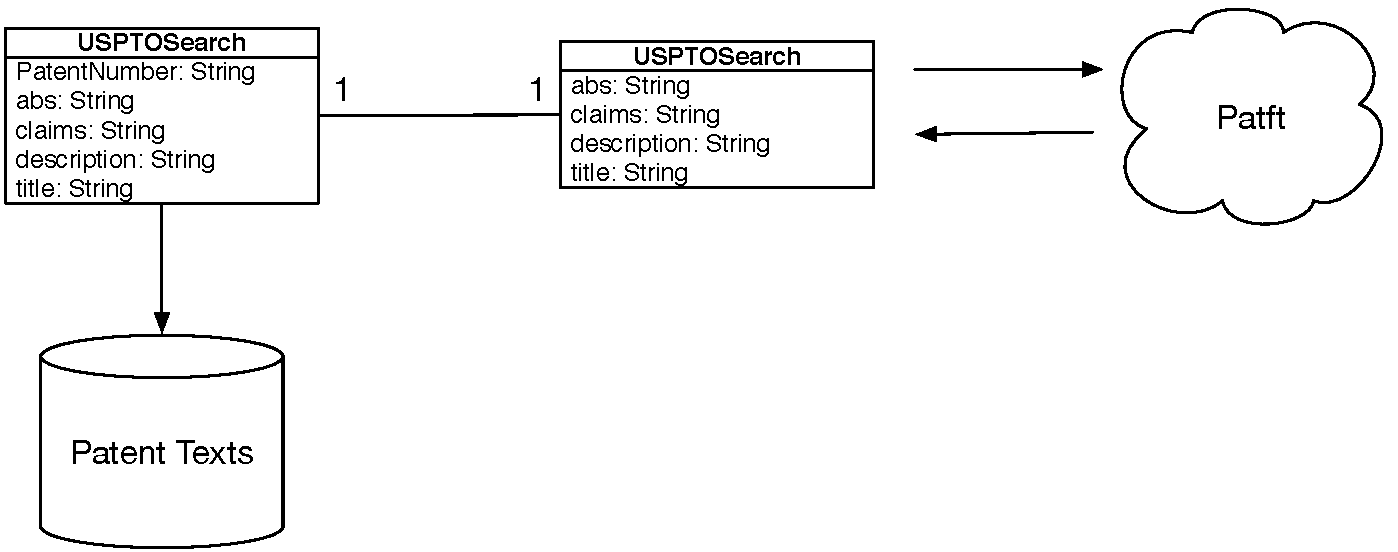
\includegraphics[scale=0.65]{TextExtractor.pdf}
\caption{the Text Extractor Part}
\end{figure}

The figure 4.11 shows the text extractor part structure. The "USPTOSearch"  accepts the patent number as a parameter. Then the "USPTOSearch" uses this number to create an instance of the "USPTOSpider". The "USPTOSpider" used the number to post a request to the USPTO patent database by using the "Patft" API. A successful response of the request is a html file of the patent document. The spider tries to find the title, the abstract, the claim, and the description and returns them to the "USPTOSearch" class. Sometimes the patent document doesn't contain these texts. For example, some old patent documents don't have digital forms of the patent documents and the scanned pictures of the patent documents are used. In addition, sometimes the API may not give a successful response due to the network problem or the server problem. In this case, the spider will try to do the request three times. If all of them fail, all the texts will be assigned  null values instead. After extracting the texts, the "USPTOSearch" class store all the texts by using special file paths for all the texts which are specialized by the patent numbers. The null value of any text will be stored as an empty string in the file. 


\subsection{the Preprocessing}
\begin{figure}
\centering
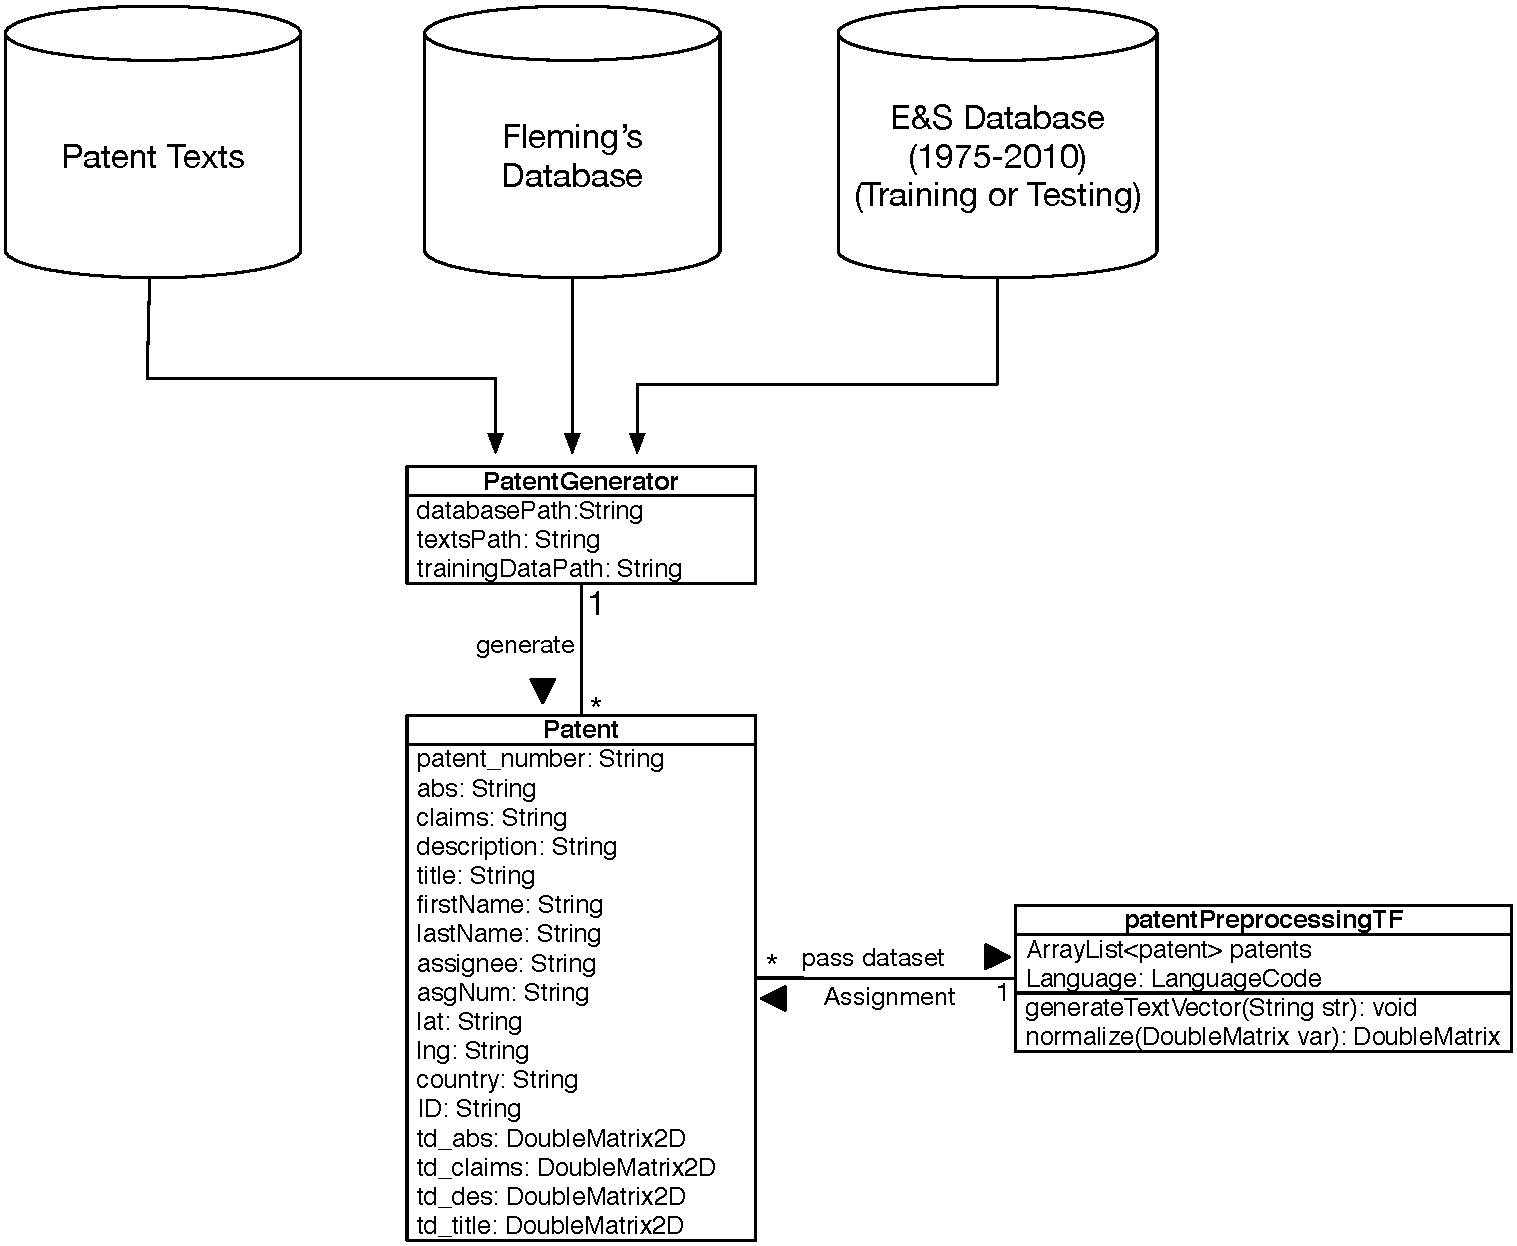
\includegraphics[scale=0.65]{preProcessing.pdf}
\caption{the Preprocessing Part}
\end{figure}
The figure 4.12 shows the preprocessing part. The part contains three classes and connects three databases. First, the patent basic information such as the inventors' names, identification information and the patent number are extracted from the E\&S database by the "patentGenerator" class. Then the "patentGenerator" class connects to the Flemming's database to extract the other information of the patents such as the assignee information and location information. After that, the "patentGenerator" class connects to the patent text dataset to extract the texts of the patent documents. With all these information, a dataset of the inventor-patent instances are generated. The inventor-patent instances are passed to the "patentPreprocessingTF" class. The "patentPreprocessingTF" mainly to do the text preprocessing.  Before doing the text preprocessing, the language of the patent document should be identified first. Because all these patents are from USPTO, the default language is English. The "generateTextVector" function performs the operations such as the removing stopwords, stemming,  term frequency counting. These operations are implemented by using the "carrot2" package. The "normalize" function is used to do a normalization on the term frequency vector. The "generatorTextVector" also uses apache math package to do the singular value decomposition to implement the latent semantic indexing. After that, the text  vector variables of the inventor-patent instances in the dataset are assigned the generated text vectors.

\subsection{the Logistic Regression}
\begin{figure}
\centering
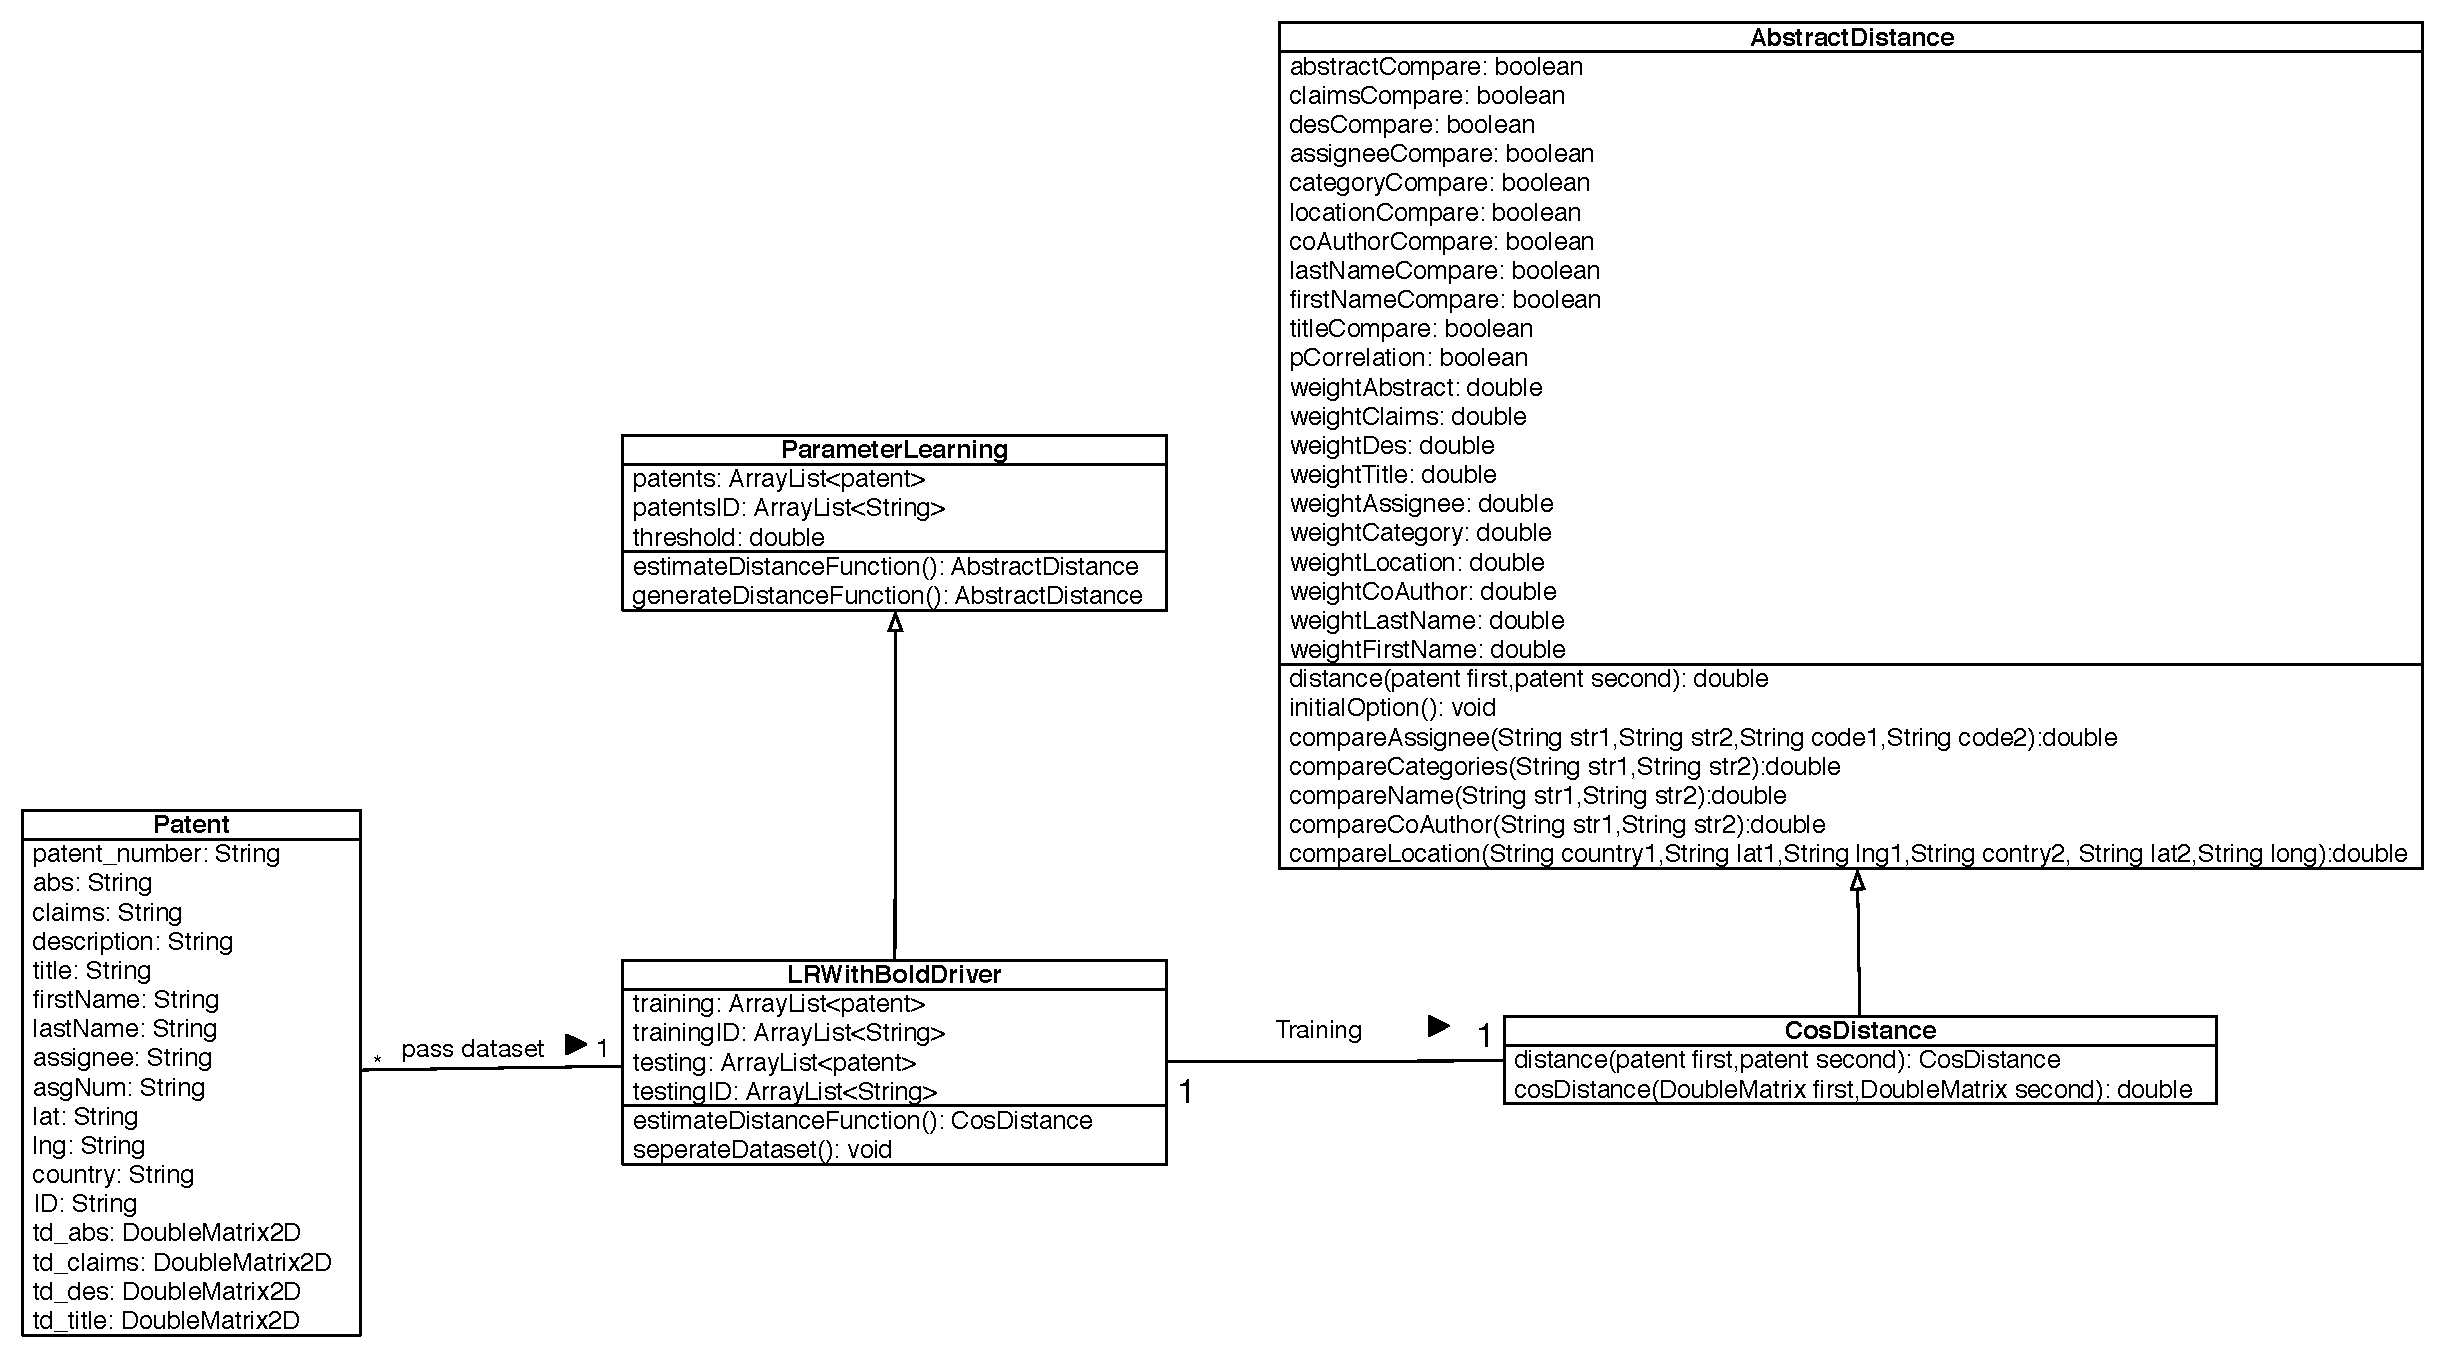
\includegraphics[width=\headwidth]{logisticRegression.pdf}
\caption{the Logistic Regression Part}
\end{figure}
After generating the inventor-patent instance dataset, this dataset is passed to the logistic regression part which is shown in figure 4.13. The main logistic regression class is "LRWithBoldDriver" class. This class has a superclass in the project called the "parameterLearning" which can be used to extend the training methods by using other techniques in the future. The "parameterLearning" class contains an arraylist of the inventor-patent instances and their inventor identification information. The "generateDistance" function is used to generate the distance function based on the training result. The "LRWithBoldDriver" class is an implementation of the logistic regression training with bold driver technique and "Stop-Early" technique. The "separateDataset" function is to divide the inventor-patent instance dataset into training dataset and the validation dataset for the "Stop-Early" technique. After the training, the suitable values are found for the weights of the features and the threshold. Based on these values, the distance function is generated. The distance function class is the "cosDistance" class which is the subclass of the "abstractDistance". The abstract class contains a list of boolean variable and double variable to identify the the features used and the weights of the features. The "pCorrelation" variable is to change the state of the distance function. If the "pCorrelation" is true, the distance function is transformed into a similarity function. The "abstractDistance" contains several functions to calculate the similarity based on different features. The "cosDistance" as a subclass adds a "cosDistance" function to calculate the similarity between two vectors. The distance function in the distance class is used to calculate the global similarity between two inventor-patent instances. The generated distance function is used by the clustering algorithms.

\subsection{the Clustering}
\begin{figure}
\centering
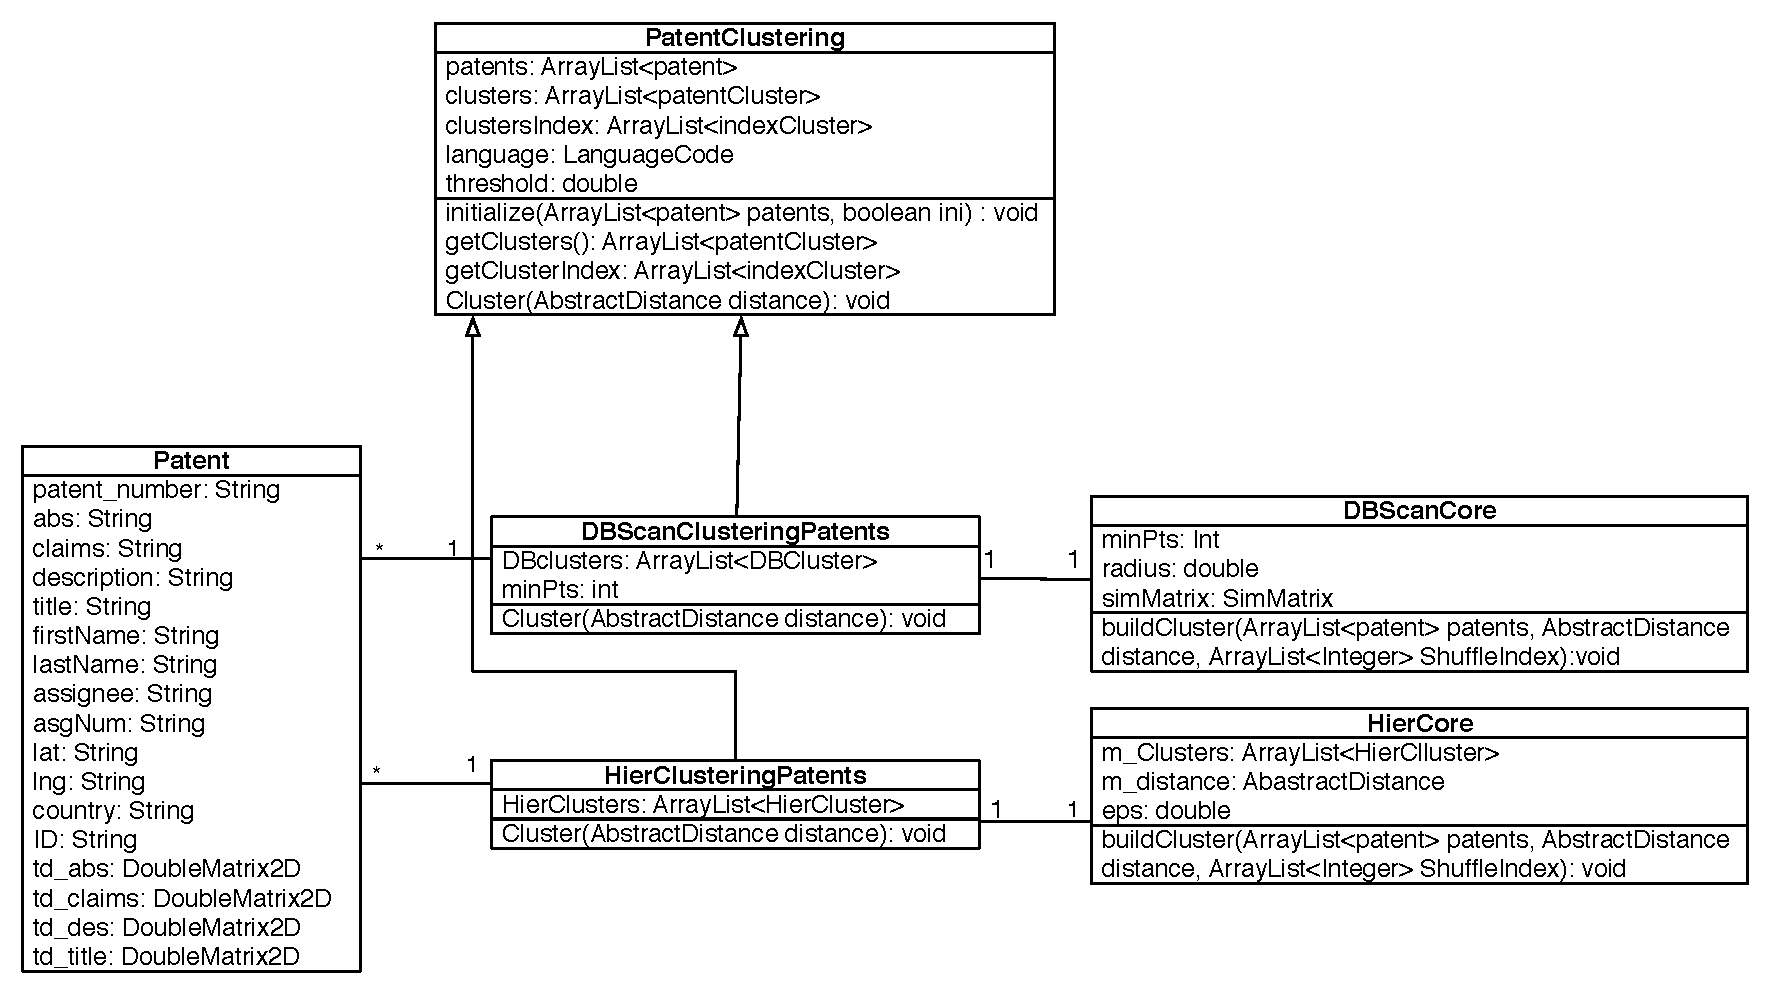
\includegraphics[width=\headwidth]{clusteringPart.pdf}
\caption{the Clustering Part}
\end{figure}
The figure 4.14 shows the structure of the clustering part. As it's explained before, the clustering of my approach contains two clustering algorithms, the hierarchical clustering and the DBSCAN. A superclass is designed for this clustering algorithms in order to extend the clustering algorithms in the future. The "patentClustering" class contains two arraylists to represent the inventor-patent instance cluster and the inventor-patent index cluster. Because sometimes in the evaluation part, the order of the inventor-patent instances should be shuffled. The index cluster is used to store the original index of the inventor-patent instances. There are two classes which are designed for both of the clustering algorithms, "DBSCANClsuteringPatents" class and the "HierClusteringPatents" class. These classes store some parameters for the clustering algorithms and different "cluster" classes are designed for them. There are two other classes are designed separately for them which are used to perform the clustering algorithms. The "DBSCANCore" class performs the DBSCAN clustering while the "HierCore" class performs the hierarchical clustering. After performing the clustering algorithm, the "DBSCANCore" and the "HierCore" classes return the clustering result  to the "DBSCANPatentClustering" and the "HierPatentClustering" classes.

\subsection{the Patent-publication Matching}
The patent-publication matching part is used to refine the clustering result to improve the accuracy. After the clustering, the inventor-patent instances are grouped into clusters. This cluster information is store into the "patentCluster" instances. The "patentCluster" class uses an arraylist to store all the inventor-patent instances. The "addPatents" function and the "getPatents" function are used to add the inventor-patent instances into the cluster and return all the inventor-patent instances. The "Refinement" class receives these clusters. The "findTheName" function is to assign a name to the cluster. The name is consists of the last name and the first letters of the first name and the middle name. The "hashSetting" function is to find the candidates to merge by checking the cluster name. If the clusters have the same name, the clusters are chosen as the candidates. Afterwords, the candidates are passed to the publication search class. The candidate names are used as the keywords to extract the publication information by using the Europe PMC API.  The API returns an xml file contained all the possible matching publication information. A web spider is designed specially for that to process the xml files. Because these xml files contain several kinds of the publication information, the "process" function is to extract the publication information individually and pass the information to the "processOneResult" function. The "processOneResult" function deals with one publication and store the publication information into a file. This information is about the abstract, the title and the affiliation and it is stored into a xml file. The "PublicationMatching" class is the core class for the patent-publication matching part. The "oneClusterMatching" is to try to find the suitable ID for one cluster by using "NPRMatching", "affiliationMatching"  and  "abstractMatching" functions.  These functions are related to the  "NPR matching method", the "Assignee-affiliation Matching method" and the "Abstract Matching method" which are mentioned before. These functions are also called in a serial order. If the previous matching method returns a ID, the rest of the matching methods will not be called any more.  After that, the "MergeCluster" function is to try to merge the clusters with the same IDs. The merged clusters of the cluster candidates and the clusters which are not chosen as the candidates consist the final result of the inventor identification.






\begin{figure}
\centering
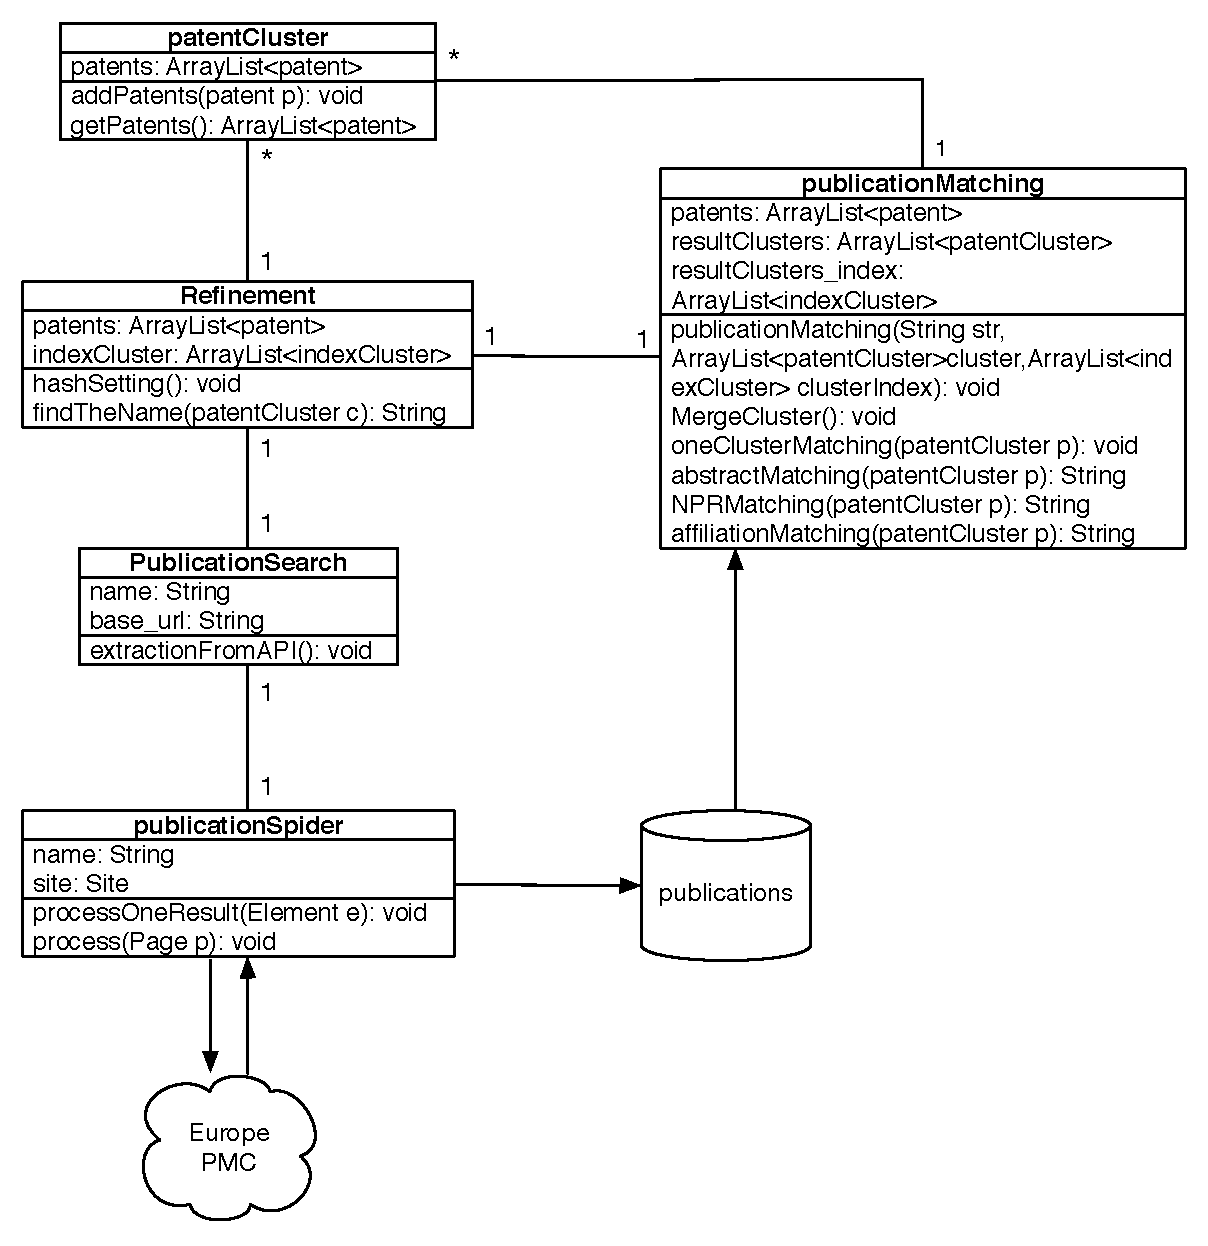
\includegraphics[width=\headwidth]{publicationMatching.pdf}
\caption{the Patent-publication Matching Part}
\end{figure}


\newpage

\subsection{the Evaluation}
 \begin{figure}
\centering
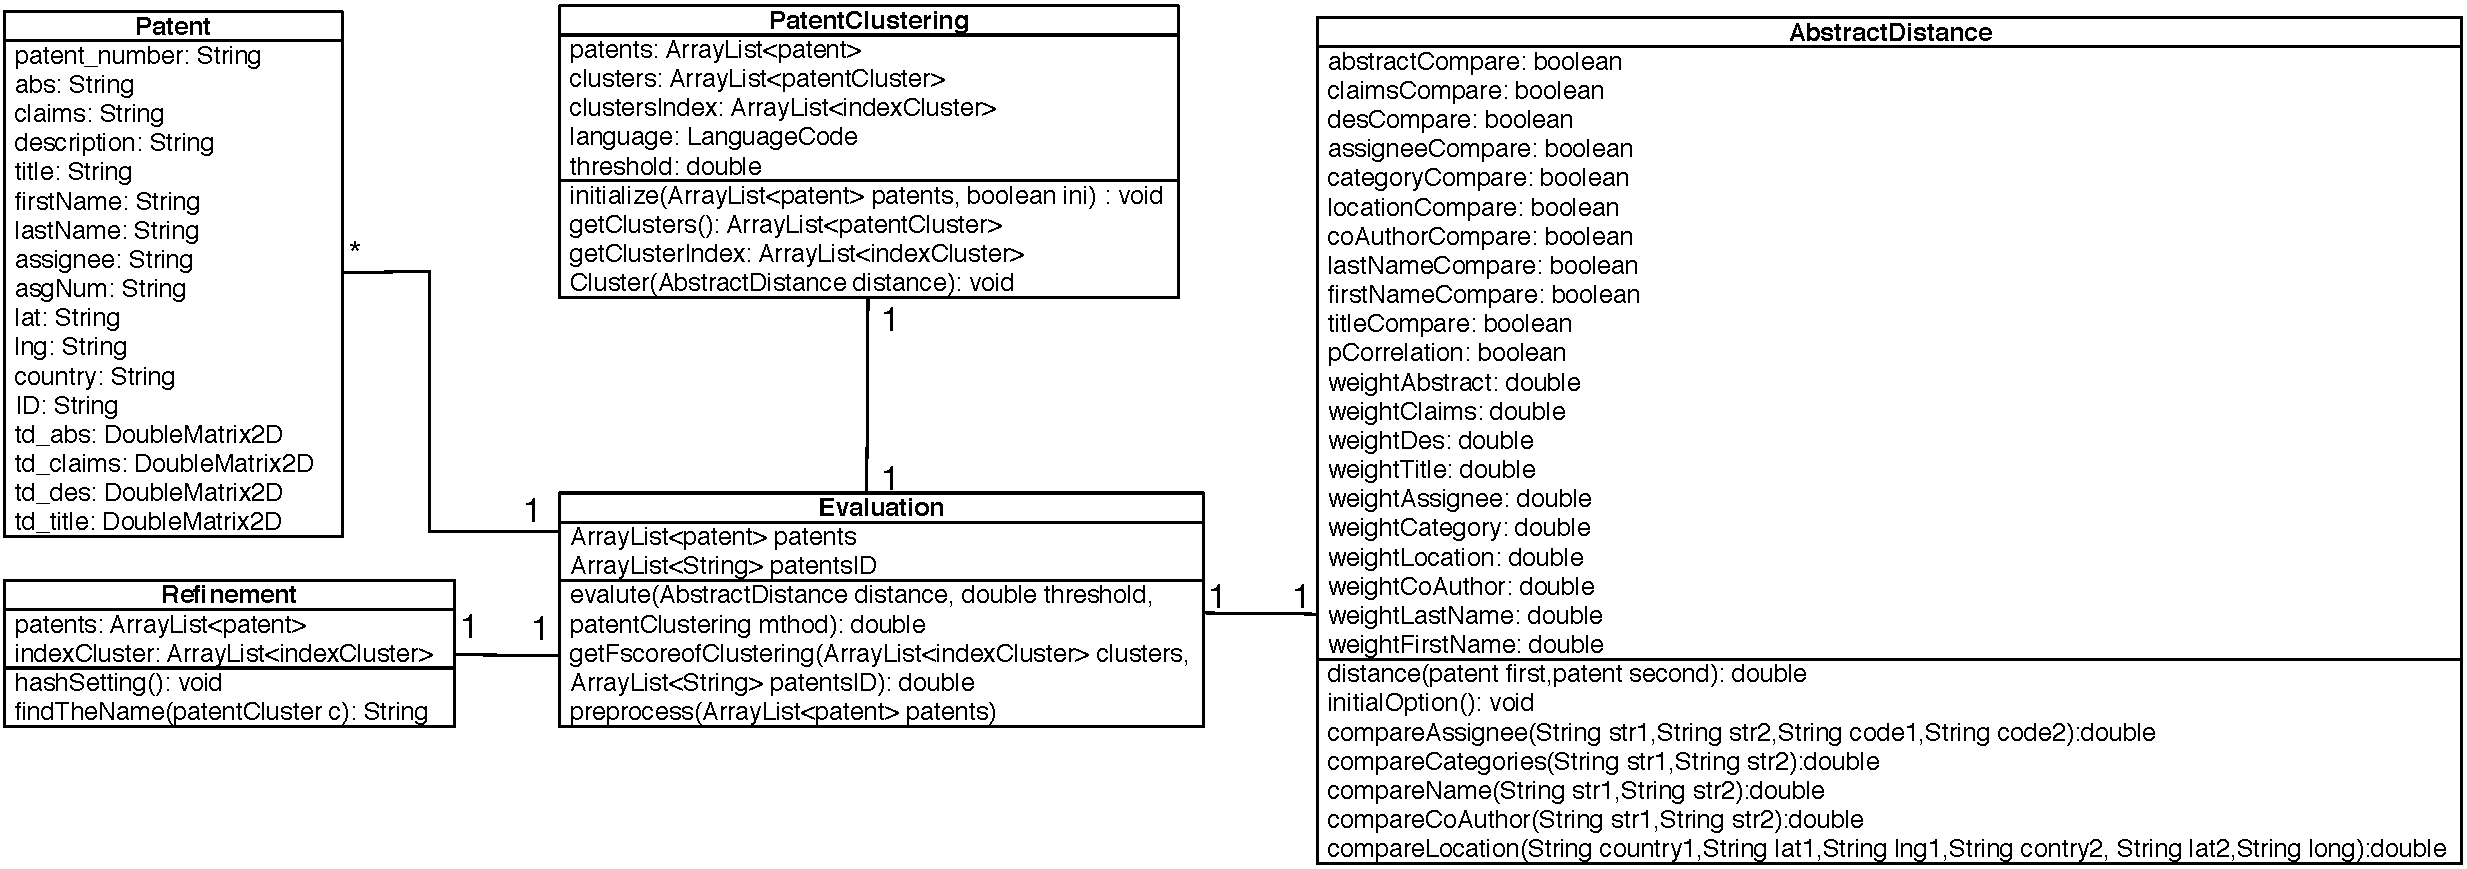
\includegraphics[width=\headwidth]{evaluation.pdf}
\caption{the Evaluation Part}
\end{figure}
Evaluation part is shown in the figure 4.16. An inventor-patent instance dataset is passed to the evaluation class. The evaluation class needs a distance class which inherits the "abstractDisntance" class. The "cosDistance" class is used in my approach. Another clustering class which needs to inherit the "patentClustering" class is also needed for the evaluation class. The "DBSCANClusteringPatents" and the "HierClusteringPatents" classes are used in my approach. The "Refinement" class  used for the evaluation is for the patent-publication matching. The evaluation class performs the clustering algorithms based on the distance function and the patent-publication matching. After that, the final clusters of the inventor-patent instances are used to evaluate the performance based on the true inventor identification information. The patent identification information is stored in the arraylist called "patentsID". The "getFscoreofClustering" function calculates the F-measure which is the main measurement for the result. The F-measure value is the default value returned by the "Evaluation" class. Another two measurements called the splitting error and lumping error are also calculated and can be accessed through the evaluation class.
 
%The USPTOSearch class is used to connect the three components, Patft API, USPTOSearch and Patent Texts dataset. The patent number is passed to the USPTOSearch as a paramter value. Based on this patent number, the USPTOSearch tries to apply a request to the USPTO patent database by using the Patft API. A successful response of the request is to return a html file of the patent document. Sometimes the Patft may not give a successful response because of the network problem or the server problem. However, the USPTOSearch wi 